\documentclass[]{article}
\usepackage{lmodern}
\usepackage{amssymb,amsmath}
\usepackage{ifxetex,ifluatex}
\usepackage{fixltx2e} % provides \textsubscript
\ifnum 0\ifxetex 1\fi\ifluatex 1\fi=0 % if pdftex
  \usepackage[T1]{fontenc}
  \usepackage[utf8]{inputenc}
\else % if luatex or xelatex
  \ifxetex
    \usepackage{mathspec}
  \else
    \usepackage{fontspec}
  \fi
  \defaultfontfeatures{Ligatures=TeX,Scale=MatchLowercase}
\fi

% use upquote if available, for straight quotes in verbatim environments
\IfFileExists{upquote.sty}{\usepackage{upquote}}{}
% use microtype if available
\IfFileExists{microtype.sty}{%
\usepackage{microtype}
\UseMicrotypeSet[protrusion]{basicmath} % disable protrusion for tt fonts
}{}
\usepackage[unicode=true]{hyperref}
\hypersetup{
            pdfborder={0 0 0},
            breaklinks=true}
\urlstyle{same}  % don't use monospace font for urls
\usepackage{graphicx,grffile}
\makeatletter
\def\maxwidth{\ifdim\Gin@nat@width>\linewidth\linewidth\else\Gin@nat@width\fi}
\def\maxheight{\ifdim\Gin@nat@height>\textheight\textheight\else\Gin@nat@height\fi}
\makeatother
% Scale images if necessary, so that they will not overflow the page
% margins by default, and it is still possible to overwrite the defaults
% using explicit options in \includegraphics[width, height, ...]{}
\setkeys{Gin}{width=\maxwidth,height=\maxheight,keepaspectratio}
\IfFileExists{parskip.sty}{%
\usepackage{parskip}
}{% else
\setlength{\parindent}{0pt}
\setlength{\parskip}{6pt plus 2pt minus 1pt}
}
\setlength{\emergencystretch}{3em}  % prevent overfull lines
\providecommand{\tightlist}{%
  \setlength{\itemsep}{0pt}\setlength{\parskip}{0pt}}
\setcounter{secnumdepth}{0}
% Redefines (sub)paragraphs to behave more like sections
\ifx\paragraph\undefined\else
\let\oldparagraph\paragraph
\renewcommand{\paragraph}[1]{\oldparagraph{#1}\mbox{}}
\fi
\ifx\subparagraph\undefined\else
\let\oldsubparagraph\subparagraph
\renewcommand{\subparagraph}[1]{\oldsubparagraph{#1}\mbox{}}
\fi

\date{}

\begin{document}
\title{TEXT AND SPEECH INTERCONVERSION}
\maketitle
\paragraph{Rakshit Kulkarni 191IT245}\label{rakshit-kulkarni-191it245}

\begin{quote}
\textbf{Information Technology}

\textbf{National Institute of Technology Karnataka Surathkal, India
575025}

\textbf{Email:
\href{mailto:rakshitkulkarni.191it245@nitk.edu.in}{\emph{rakshitkulkarni.191it245@nitk.edu.in}}}

\textbf{Kiran Kumar J M 191IT126}

\textbf{Information Technology}

\textbf{National Institute of Technology Karnataka Surathkal, India
575025}

\textbf{Email:
\href{mailto:kirankumarjm.191it126@nitk.edu.in}{\emph{kirankumarjm.191it126@nitk.edu.in}}}

\textbf{Mohit Awachar 191IT231}

\textbf{Information Technology}

\textbf{National Institute of Technology Karnataka Surathkal, India
575025}

\textbf{Email:
\href{http://mohit.191it231@nitk.edu.in/}{\emph{mohit.191it231@nitk.edu.in}}}

\textbf{Anshul Patel 191IT208}

\textbf{Information Technology}

\textbf{National Institute of Technology Karnataka Surathkal, India
575025}

\textbf{Email:
\href{mailto:anshupatel.191it208@nitk.edu.in}{\emph{anshupatel.191it208@nitk.edu.in}}}

\textbf{ABSTRACT:}

We built two Applications (TTS \& STT) for interconversion between text
and speech signal. Text to speech makes the online world and beyond
available to people with learning disabilities, visual impairments, and
literacy challenges. While speech to text saves a lot of typing time.
Two separate Graphic User Interfaces (GUI) are built of these tasks
using python tkinter library. TTS applications turn text-based content
into audio and enable all users to access information and communicate
with others. While STT does the reverse. The SST module also allows
searching converted text on the web(Google Search). We use python's
pysttx3 library for TTS and python's speech\_recognition library for STT
respectively.Active internet connection is needed for speech to text
conversion.
\end{quote}

\section{Keywords:}\label{keywords}

\begin{quote}
Communication, FreeTTS, FreeSST, python, pysttx3, tkinter, Speech,
Text-To-Speech, Speech-To-Text , speech\_recognition
\end{quote}

\section{\texorpdfstring{\\
INTRODUCTION:}{ INTRODUCTION:}}\label{introduction}

\begin{quote}
Text-to-speech (TTS) convention transforms linguistic information stored
as data or text into speech. It is widely used in audio reading devices
for blind people now a days .Audiobook is one of many application of
TTS.In recent times, the use of text-to-speech conversion has grown far
beyond the disabled community to become a major adjunct to the rapidly
growing use of digital voice storage for voicemail and voice response
systems. Also developments in Speech synthesis technology for various
languages have already taken place. On other hand, Speech-To-Text (SST)
converts speech signal to text signal. Main applications for this
conversion are online assistants( Google Assistant, Siri, etc.). SST can
save a lot of energy and time required for typing. Authors can use this
for writing books, journals, etc.

TTS and STT both are useful in many areas like banking-finance sector
,ATM, healthcare, learning , publish-media etc.But we have selected this
topic mainly focussing on two sectors namely EDUCATION and HEALTH .We
choose this problem is due to its wide

application in remote areas and health sector. We build the application
with limited resources available with us here we want to show its usage
and expand its availability. We wanted to limit use of the internet so
that it can be useful in remote areas. It can be useful to areas like
hospitals where with just this application they can inform the
information to each and every patient. In situations like pandemic this
can play a vital role for spreading news or any notice to anywhere(not
restricted to hospital,can also be in places like a civil court,police
station etc) without using a piece of paper or pen as it may cause
spread of the pandemic disease. Apart from this it can make life easier
for people with disabilities. In India if we can implement this simple
idea in any school(normal or schools for disabled) then it may help them
to learn things and share their point of views without any problem and
hesitations.Along with this it can also make their life easy , smoothing
and self confident.TTS is very beneficial for blind students while SST is
very useful for deaf students. For all this problem on ground level
there is no such prominent solutions are visible in our day to day
life.By introducing this idea among deaf people where they were using
old methods(like sign language) or in hospitals(old pen-paper technique)
it can create a great impact in their lives.We are not here ensuring
that this is the only 100\% effective solution but then also we have
tried make it a light user friendly GUI which is not going to use
internet to convert text to speech.Also the speech i.e audio file will
also get stored in the system itself so that record can be maintained
for audio files. On other hand speech to text requires active internet
connection.
\end{quote}

\section{LITERATURE SURVEY:}\label{literature-survey}

\begin{quote}
During this project we analysed and understood the concepts for speech
to text conversion and for vice-versa.We also learned about various
libraries of python which made possible to create GUI for our idea and
application.For this we searched various websites,videos and papers for
the useful content.

Some of the websites which made our work easier are:
\end{quote}

\begin{itemize}
\item
  \emph{h}
  \href{https://www.tutorialspoint.com/python/python_gui_programming.htm}{\emph{ttps://www.tutorialspoint.com/python/python}}
\end{itemize}

\begin{quote}
\emph{\_}
\href{https://www.tutorialspoint.com/python/python_gui_programming.htm}{\emph{gui\_programming.htm}}:
This site also helps us to know how to add a widget and what are its
types.
\end{quote}

\begin{itemize}
\item
  \emph{h}
  \href{https://docs.python.org/3/library/tkinter.html}{\emph{ttps://docs.python.org/3/library/tkinter.html}}:
  We used this site to know about the arguments which are present in the
  method.
\end{itemize}

\begin{quote}
Eg:-btn.place(x= ,y= ) etc..
\end{quote}

\begin{itemize}
\item
  \emph{h}
  \emph{\href{https://www.geeksforgeeks.org/python-gui-tkinter/}{ttps://www.geeksforgeeks.org/python-gui-tkint}
  e}
  \href{https://www.geeksforgeeks.org/python-gui-tkinter/}{\emph{r/}}:
  We used this site to go-through how the widget works and mainly how to
  create buttons, how to change background color etc..
\item
  \emph{h}
  \href{https://www.studytonight.com/tkinter}{\emph{ttps://www.studytonight.com/tkinter}}:
  We used this site to learn about python tkinter library and also how
  to create a GUI and how to add a widget and all the things we learnt
  from this.
\item
  \emph{h}
  \emph{\href{https://www.youtube.com/playlist?list=PLCC34OHNcOtoC6GglhF3ncJ5rLwQrLGnV}{ttps://www.youtube.com/playlist?list=PLCC34O}
  H}
  \href{https://www.youtube.com/playlist?list=PLCC34OHNcOtoC6GglhF3ncJ5rLwQrLGnV}{\emph{NcOtoC6GglhF3ncJ5rLwQrLGnV}}:
  This is a YouTube playlist on Comedy channel for tutorial of tkinter.
\end{itemize}

\begin{quote}
AGer going through 5 research papers we liked the paper which made TTS
using java and modifying it ,similarly we use python instead of java.
Ifeanyi Cosmas Nwakanma

,Ikenna Oluigbo and Okpala Izunna were the authors for the paper titled
TTS and got published on 5,MAY 2014 in International Journal of Research
in Information Technology(IJRIT)
\end{quote}

\section{Problem Statement}\label{problem-statement}

\begin{quote}
Build text to speech and speech to text synthesizer separately. Save
corresponding text file in computer. Implement voice change(male/female),
output voice speed and other necessary features in text to speech.
Implement web search of converted text in speech to text.
\end{quote}

\subsubsection{OBJECTIVES}\label{objectives}

\begin{quote}
The specific objectives are:
\end{quote}

\begin{itemize}
\item
  To enable the deaf and dumb to communicate and contribute to the
  growth of an organization through synthesized voice.To enable the
  blind and elderly people enjoy a User-friendly computer interface.
\item
  To provide an effective tool to spread information without using pen or
  paper in various places like hospitals,schools etc.
\item
  Convert text to speech without the internet so that all the above
  objectives can be achieved
\end{itemize}

\begin{quote}
even in remote areas,also to keep record of all the audio and text files.
\end{quote}

\begin{itemize}
\item
  Save typing time using speech to text and web search spoken words and
  implement Google search.
\end{itemize}

\subsubsection{METHODOLOGY:}\label{methodology}

\begin{quote}
\textbf{TTS:}

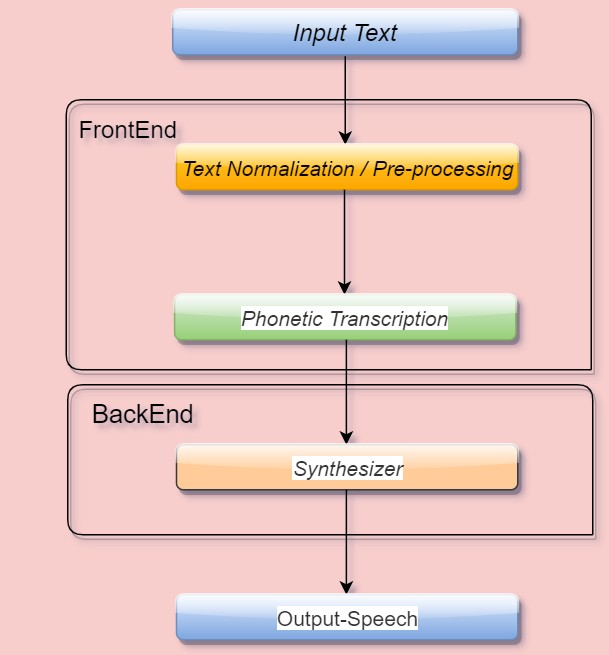
\includegraphics[width=2.69289in,height=2.11510in]{image1.jpeg}

\textbf{Input Text}: Our Text-To-Speech GUI contains mainly two types of
input Options i.e the first one is the user can import the text nothing
but .txt extension file from any directory of his/her device.And also the
another option is user can enter anything in the given text box so that
it can be converted to speech.Text language must be English.

\textbf{Front-End: Text Normalization / Pre Processing}:The front end
does two functions, the first of which is to convert raw text containing
symbols, such as, number and abbreviations into equivalent words.This
process is termed as normalization or pre-processing or tokenization. As
part of a text-to-speech (TTS) system, the text normalization component
is typically one of the first steps in the pipeline, converting raw text
into a sequence of words, which can then be passed to later components
of the system, including word pronunciation, prosody prediction, and
ultimately waveform generation.

\textbf{Phonetic Transcription} : The second function is to assign
phonetic transcription to each word. The front end converts each
phonetic until of the text into units like phrase, clauses and
sentence.This process of assigning phonetic transcription to words is
called text-to-phoneme conversion. Phonetics transcription and prosody
information together will form the symbolic linguistics
representation.The front interfaces always engage with phonetic
conversion to each unit, and divides and marks to form a speech tree or
pattern tree using the speech unit which configures the tune and rhythm
through phrases, clauses, and sentences. This process of transcription
is known as text-to-phoneme (TTP) or grapheme-to-phoneme (GTP)
conversion.

\textbf{Back-End: Synthesizer} : The back-end---oGen referred to as the
synthesizer---then converts the symbolic linguistic representation into
sound. The back-end will also include the computation of the target
prosody such as pitch counter, phoneme duration which are then imposed
speech output.The Text can be converted to speech using pyttsx3.It is a
text-to-speech conversion library in Python.It uses native speech
drivers when available and works completely offline.

\textbf{Output Speech}: AGer pre-processing and synthesis of text the
speech is generated.The speech is the output in this Text-To-Speech GUI.

\textbf{STT:}
\end{quote}

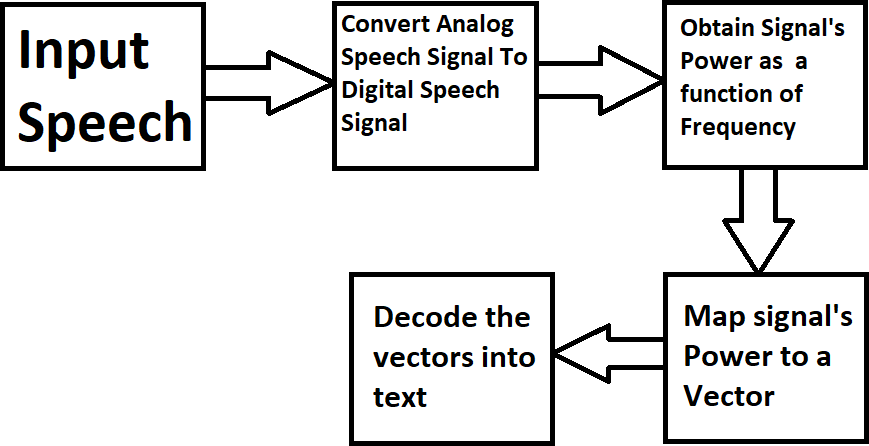
\includegraphics[width=2.58926in,height=1.20792in]{image2.png}

\begin{quote}
\textbf{Input Speech:} Speech signal is inputted from the user using a
microphone on the device.Allow Since the surrounding noise may vary, we
allow the program a second or too to adjust the energy threshold of
recording so it is adjusted according to the external noise level. This
is done using

\textbf{Convert Speech to Text:} We use recognise\_google() for this.
It's working is as follows.Voice activity detectors (VADs) are used to
reduce an audio signal to only the portions that are likely to contain
speech. This prevents the recognizer from wasting time analyzing
unnecessary parts of the signal. Speech must be converted from physical
sound to an electrical signal with a microphone, and then to digital
data with an analog-to-digital converter. Once digitized, the signal's
power is obtained as a function of frequency. Then it is mapped to a
vector of real numbers.To decode the speech into text, groups of vectors
are matched to one or more phonemes---a fundamental unit of speech.

\textbf{Output the text:} Output is produced on text box in the
application

\textbf{Google search speech(if needed):} If user asks to search the
resluted text in internet, this is done by clicking on Google symbol
which essentially gets contents in text box and search it in Google
using open\_new\_tab() function in webbrowser library.
\end{quote}

\section{RESULTS AND ANALYSIS:}\label{results-and-analysis}

\begin{quote}
\textbf{TTS}
\end{quote}

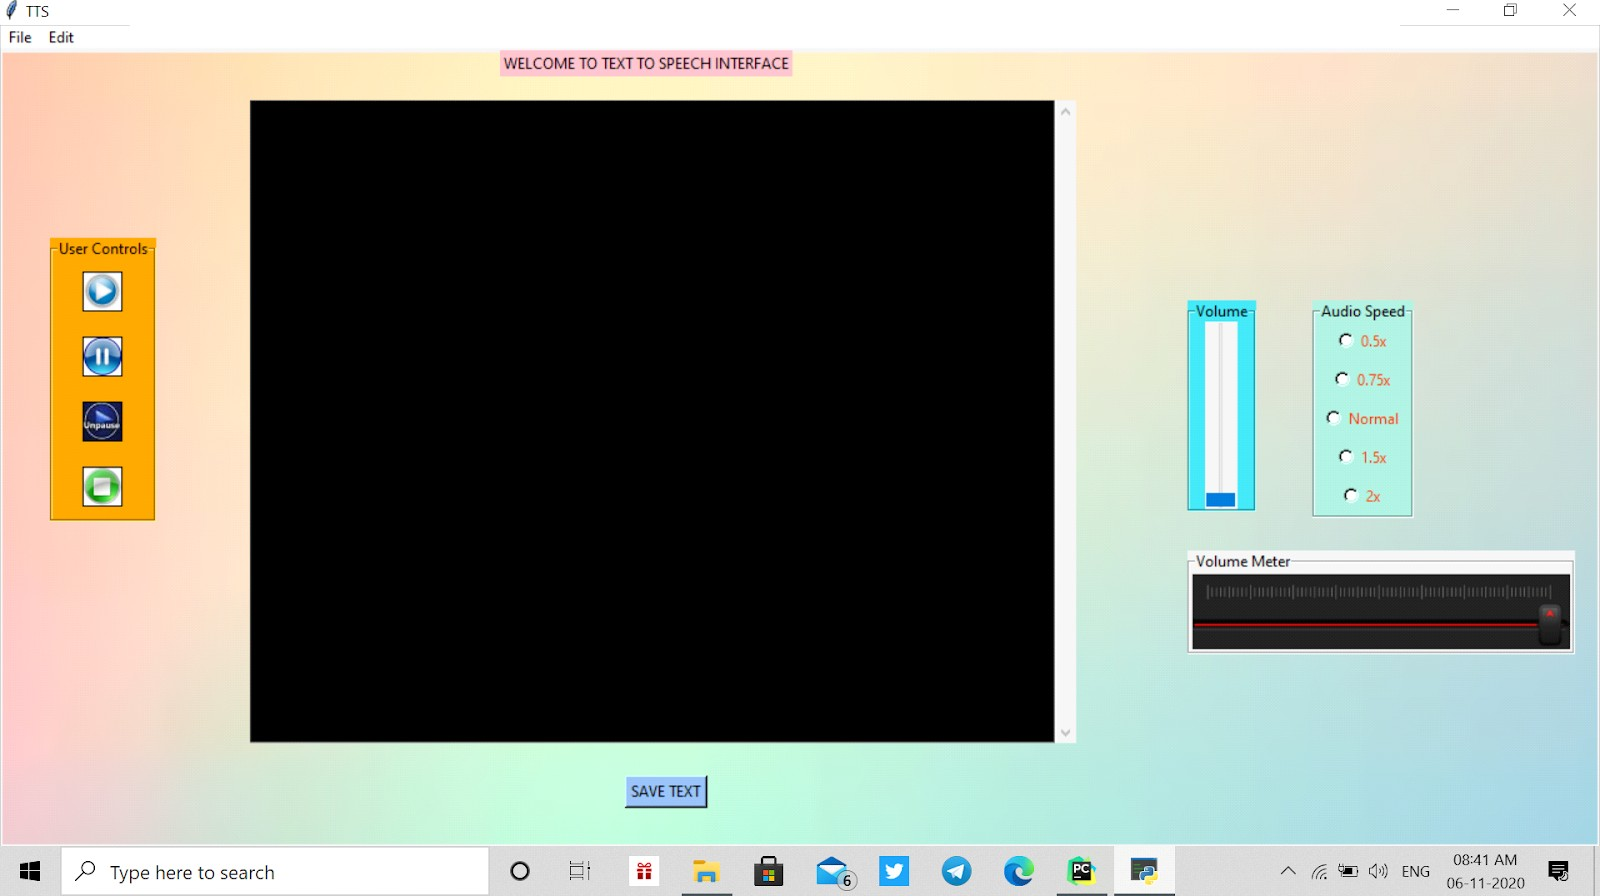
\includegraphics[width=3.16112in,height=2.05333in]{image3.jpeg}

\begin{quote}
This is our Text To Speech Graphical User Interface(GUI) which consists
of a widget like text field, Buttons, Slider, RadioButton and Menu Bar,
Label Frame, etc. By using all the widget we made a GUI which converts
Text-To- Speech.
\end{quote}

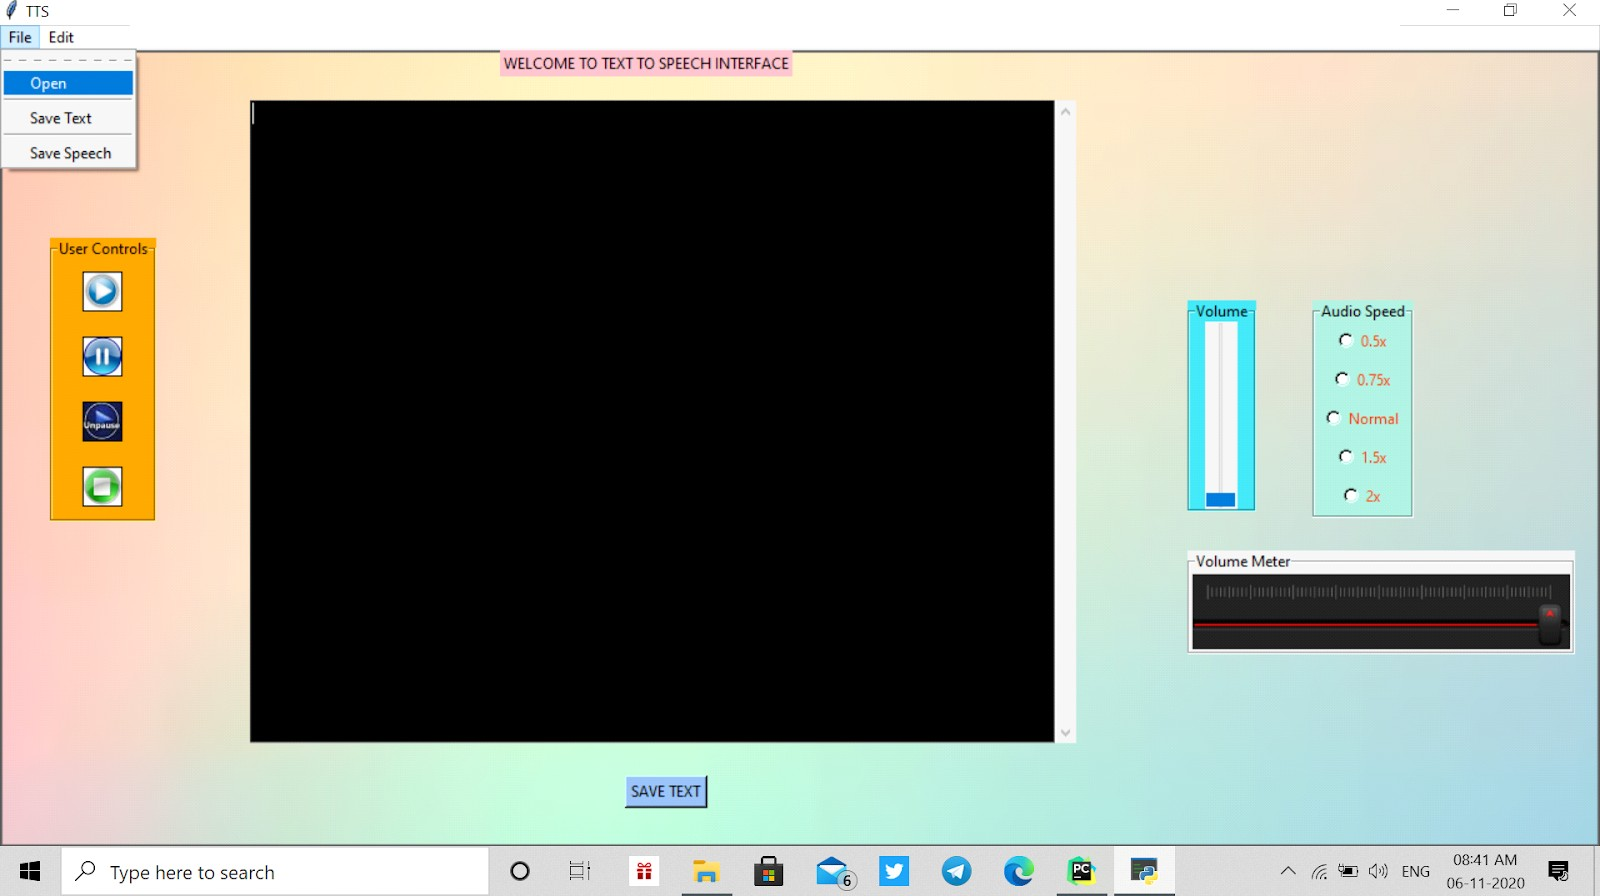
\includegraphics[width=2.96271in,height=1.86667in]{image4.jpeg}

\begin{quote}
We can input Text in Text Field in two different ways.In that First way
is by opening a text file(.txt) from the device.In the above Figure you
can see there is a file menu bar which consists of an open command to
open text(.txt) file.
\end{quote}

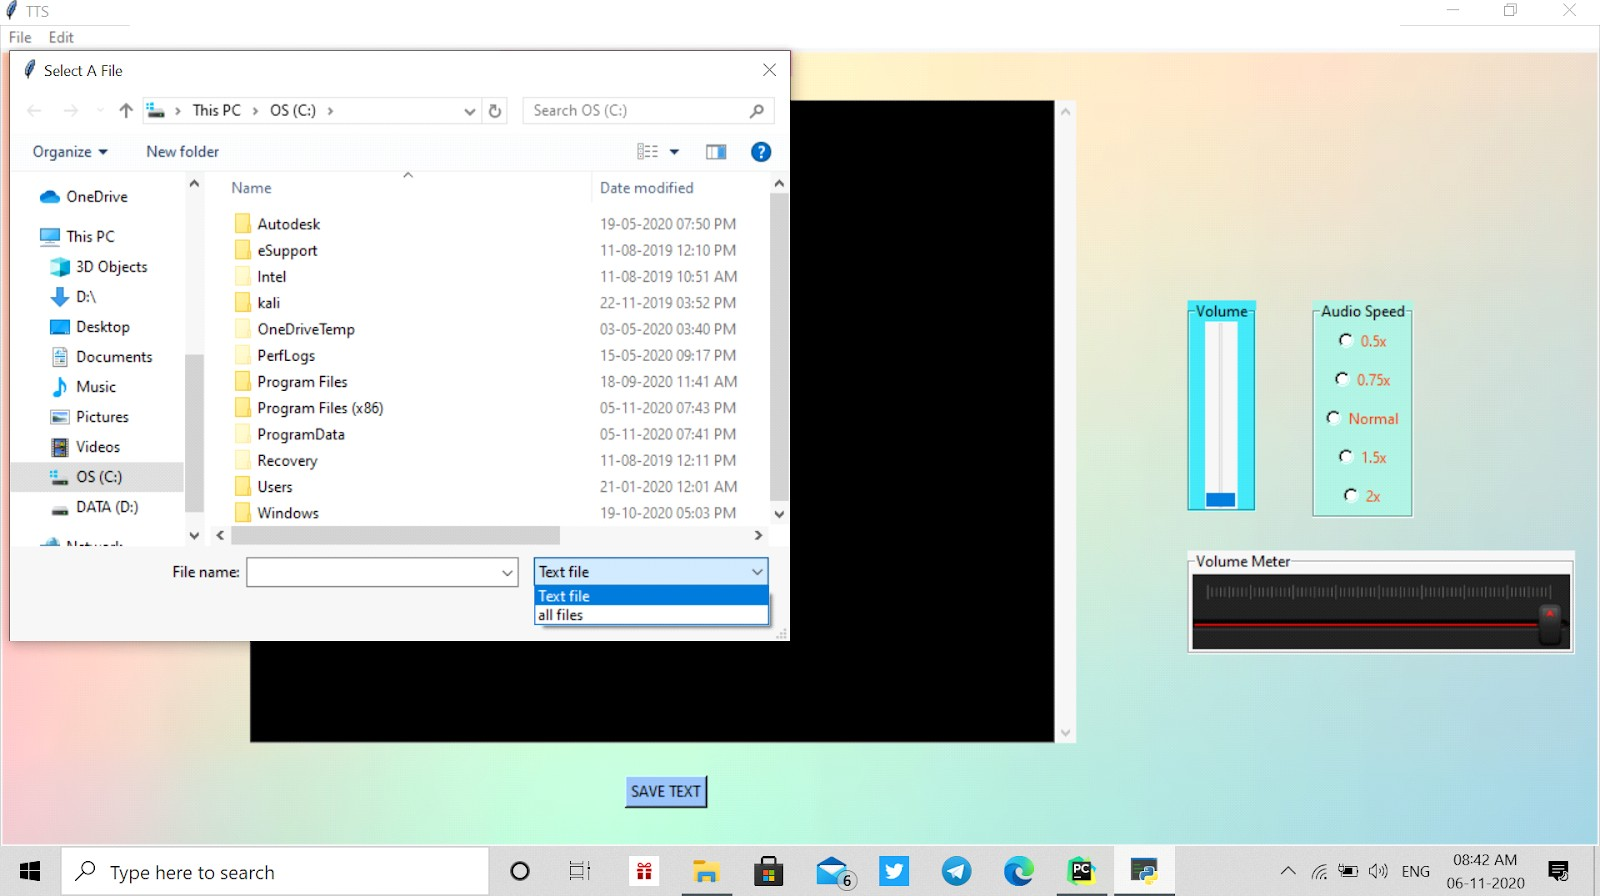
\includegraphics[width=3.03209in,height=1.96000in]{image5.jpeg}

\begin{quote}
AGer clicking on the open command you can see there is another window
named Select A File is opened.Using this we can select any text file from
any directory.

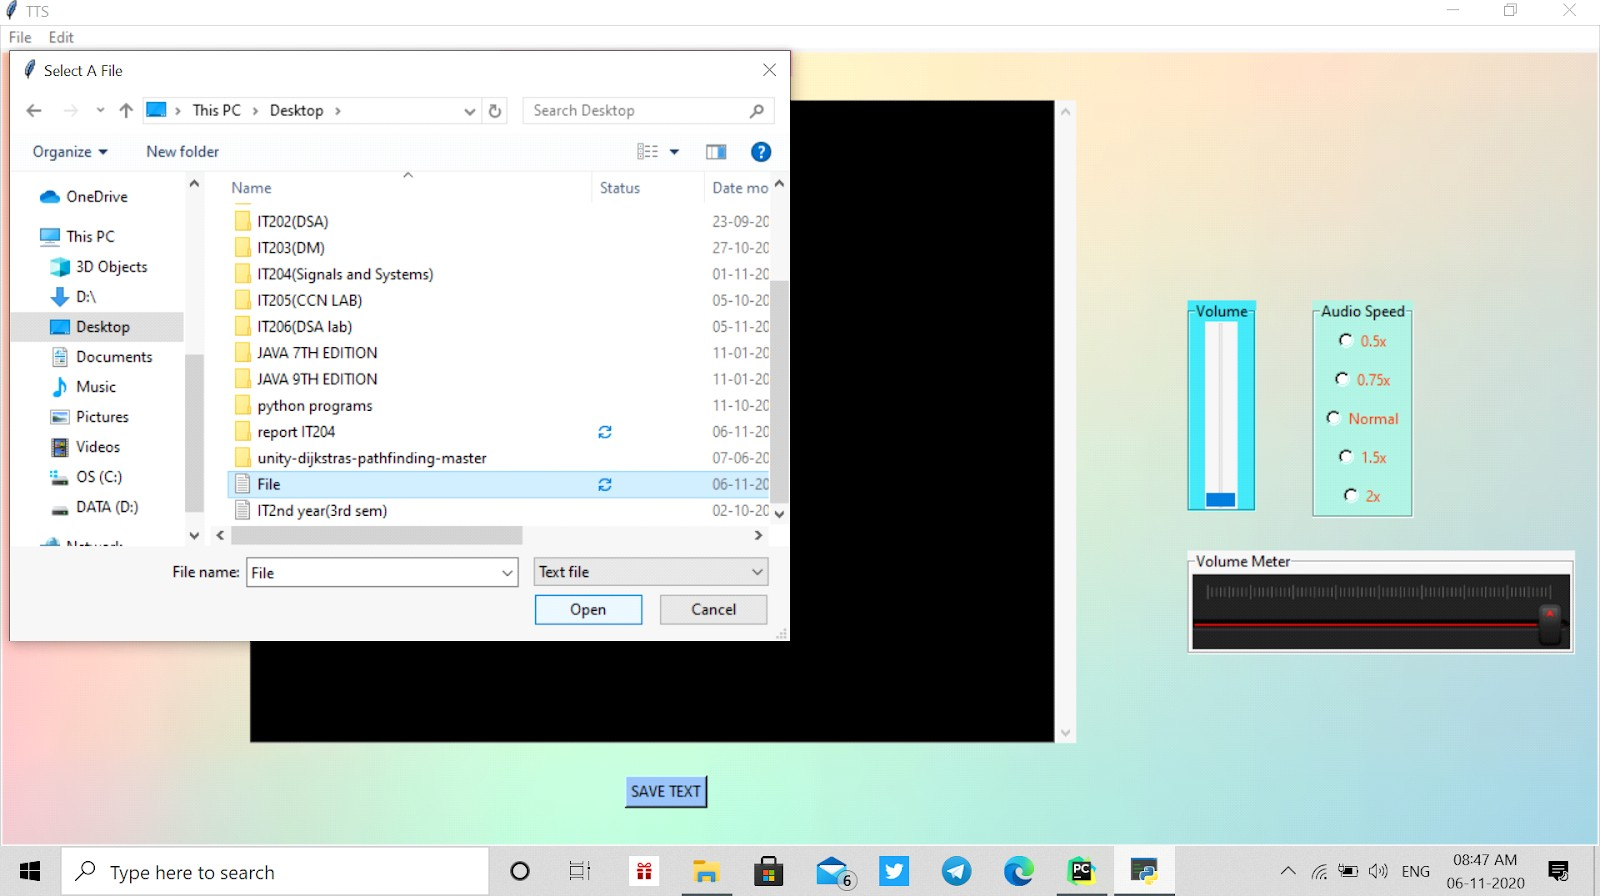
\includegraphics[width=3.14441in,height=1.68000in]{image6.jpeg}

AGer selecting a text file(.txt) click on the open button in the Select A
File named window to copy the content from the selected text file(.txt)
to the Text Field which is in the TTS named window.
\end{quote}

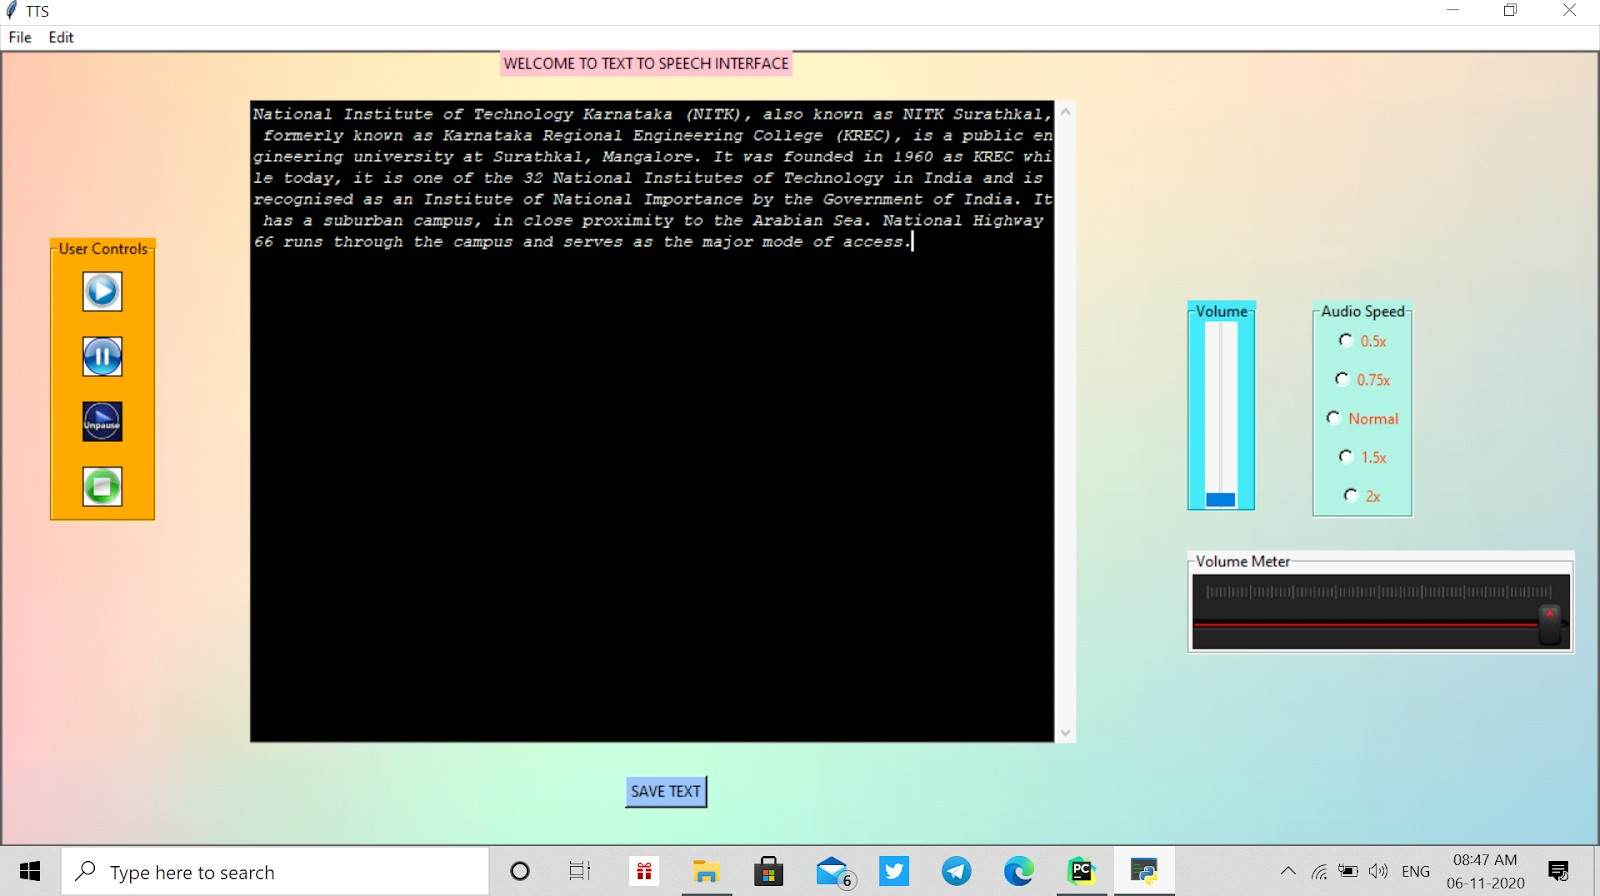
\includegraphics[width=2.99621in,height=1.77333in]{image7.jpeg}

\begin{quote}
The Content from the selected text file(.txt) is copied into the Text
field.
\end{quote}

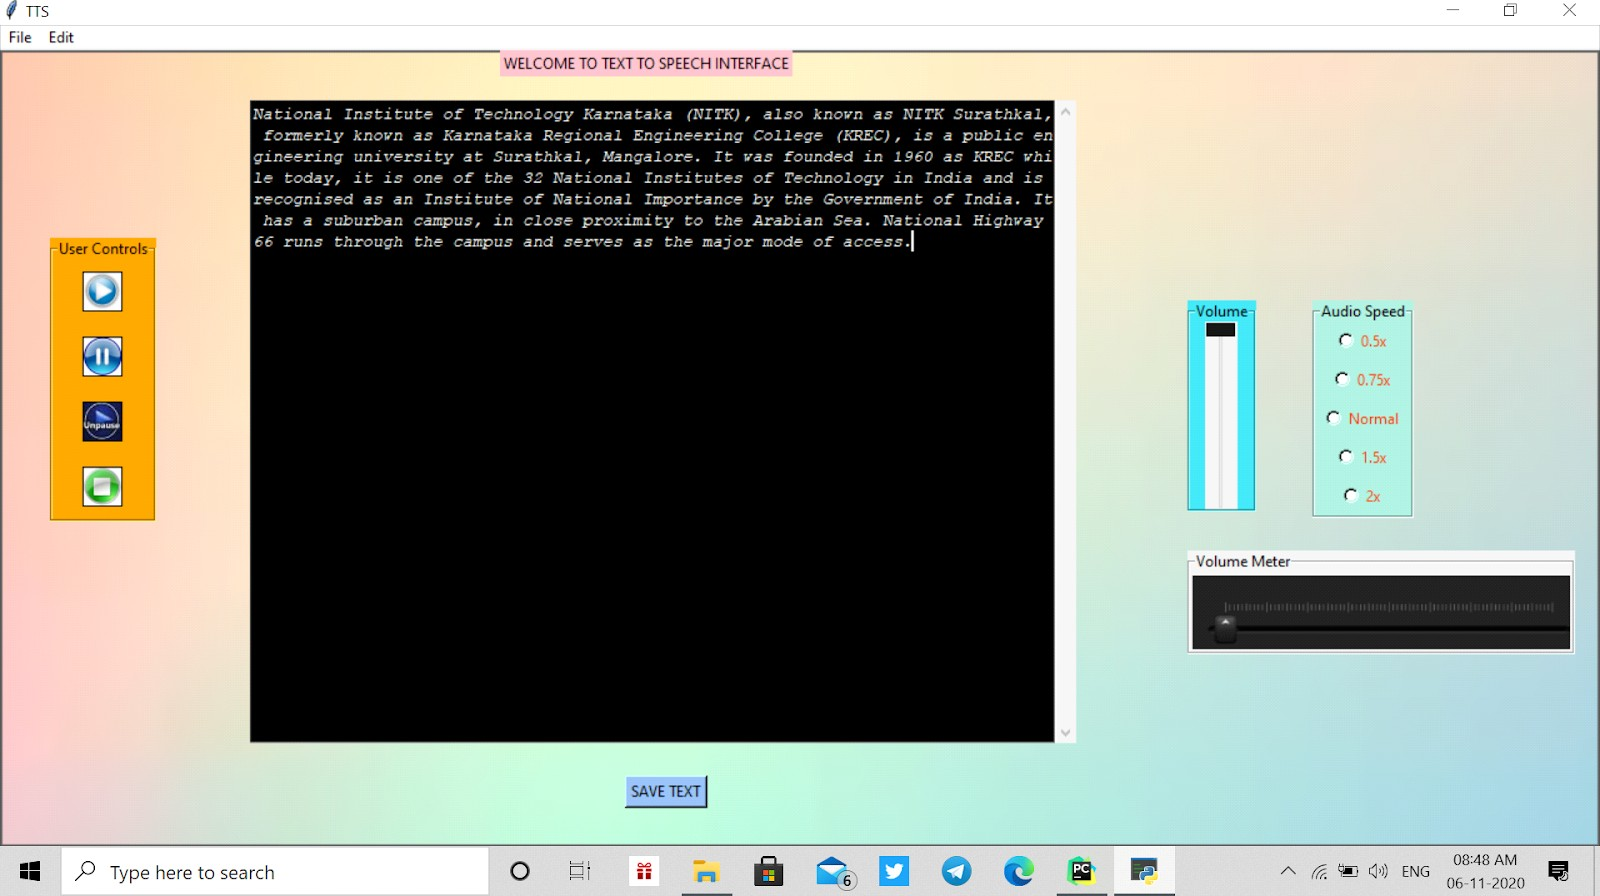
\includegraphics[width=3.06218in,height=2.05333in]{image8.jpeg}

\begin{quote}
AGer copying the content by clicking on play button which is present in
user control labelFrame to start the speech.Click on Pause button to
pause the speech,unpause button to unpause the speech and stop button to
stop the speech. And on the right side you can see Volume LabelFrame
which is used for increasing or decreasing the volume.The volume is
corresponding to the volume meter where you can see if volume is low
then in the volume meter the pointer is towards the leG.

Below images show how the pointer changes according to volume.

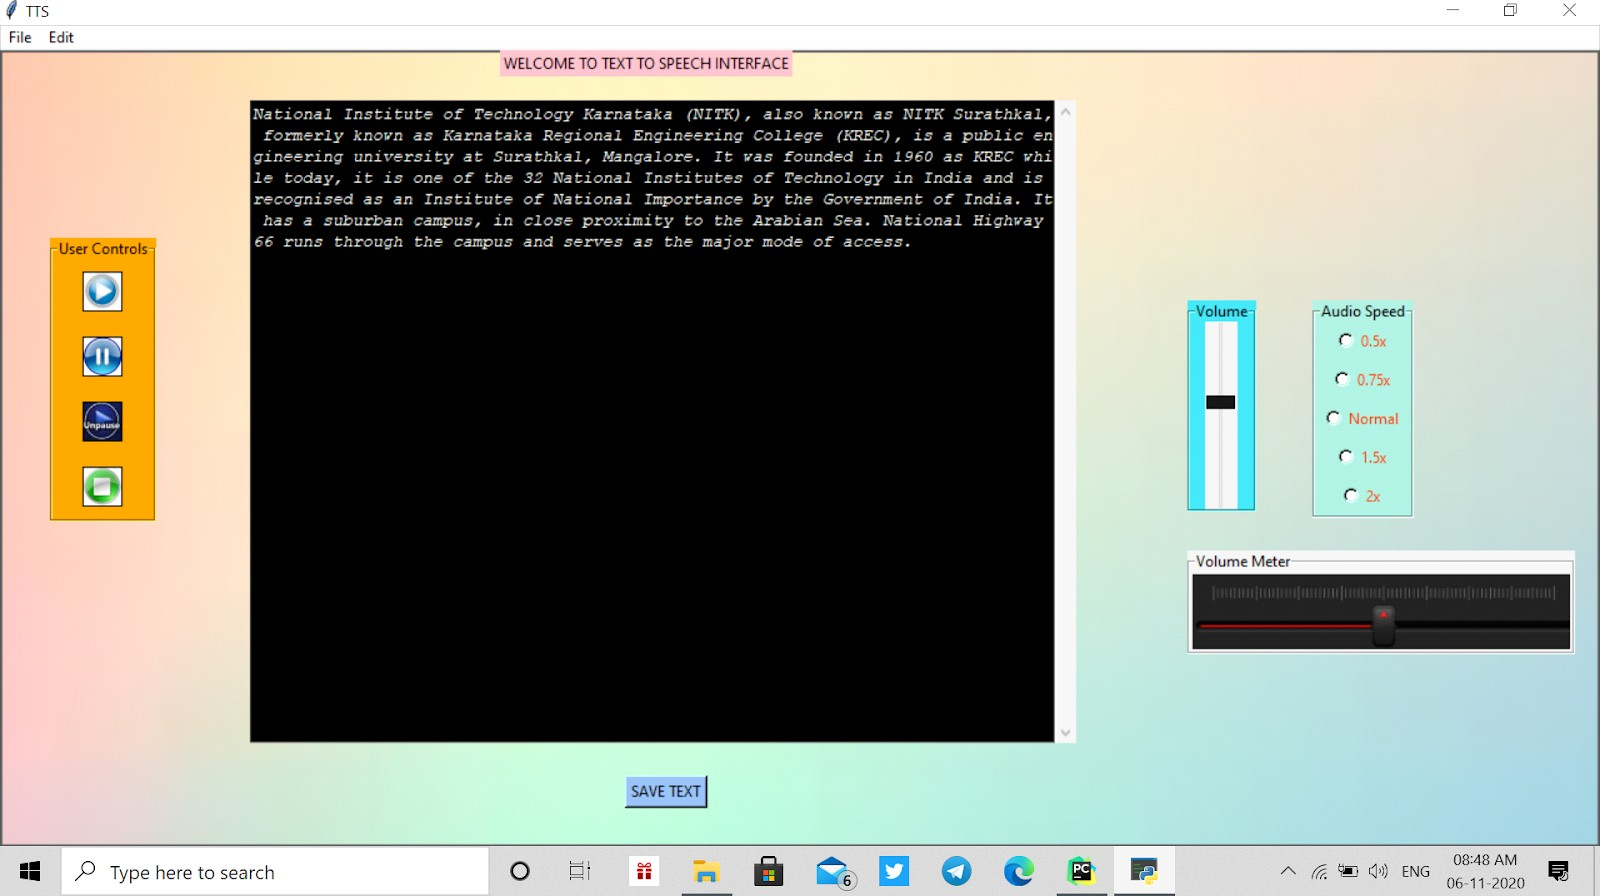
\includegraphics[width=3.06417in,height=1.77333in]{image9.jpeg}
\end{quote}

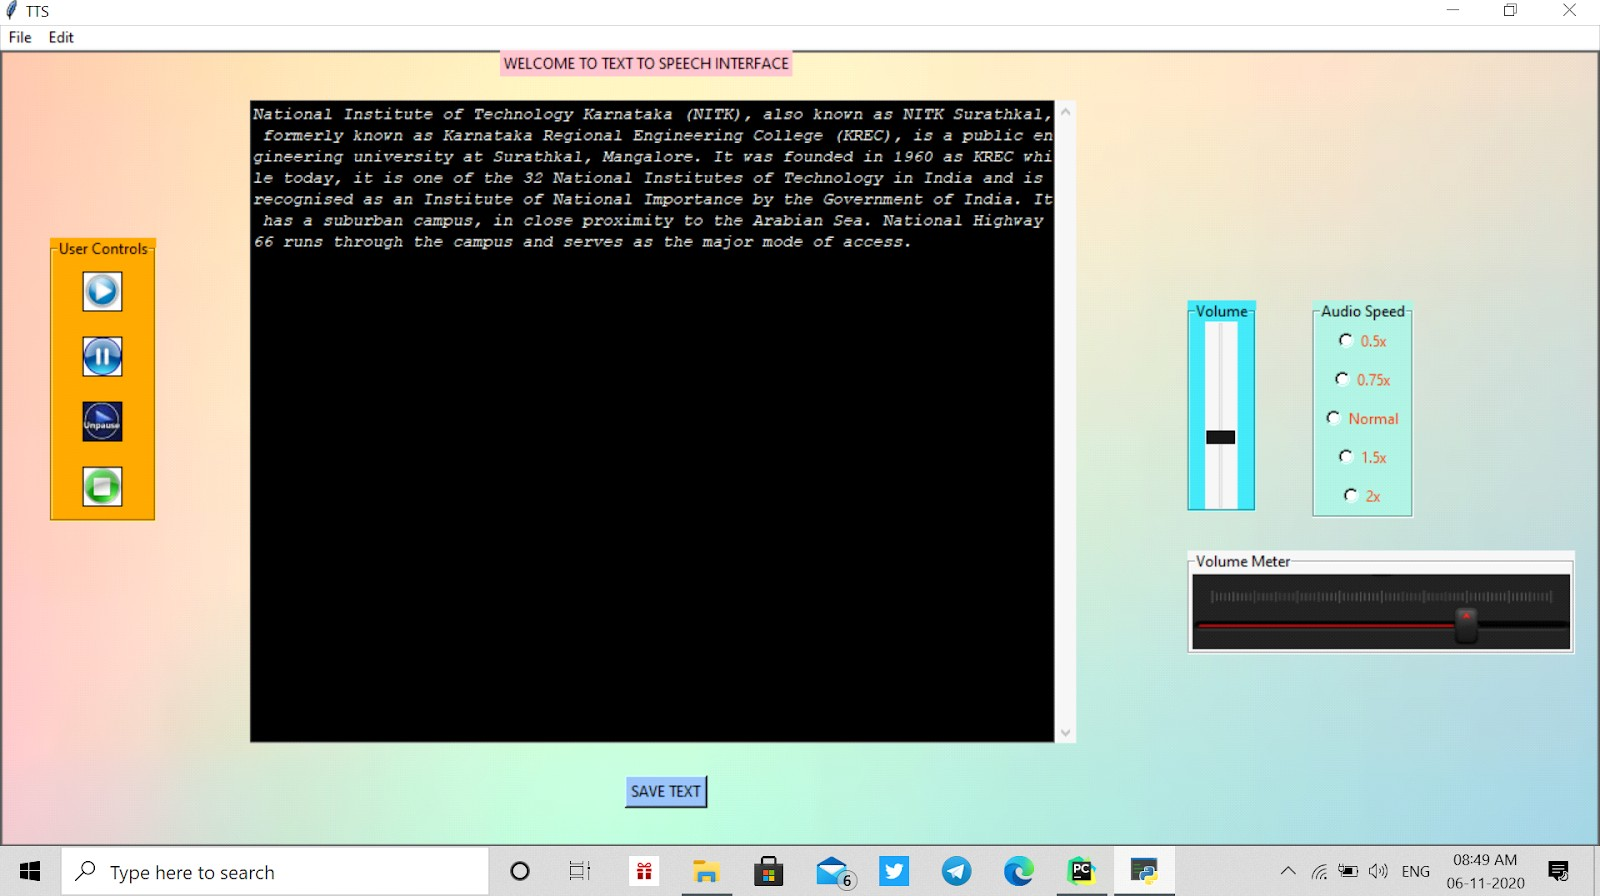
\includegraphics[width=2.97614in,height=1.68000in]{image10.jpeg}

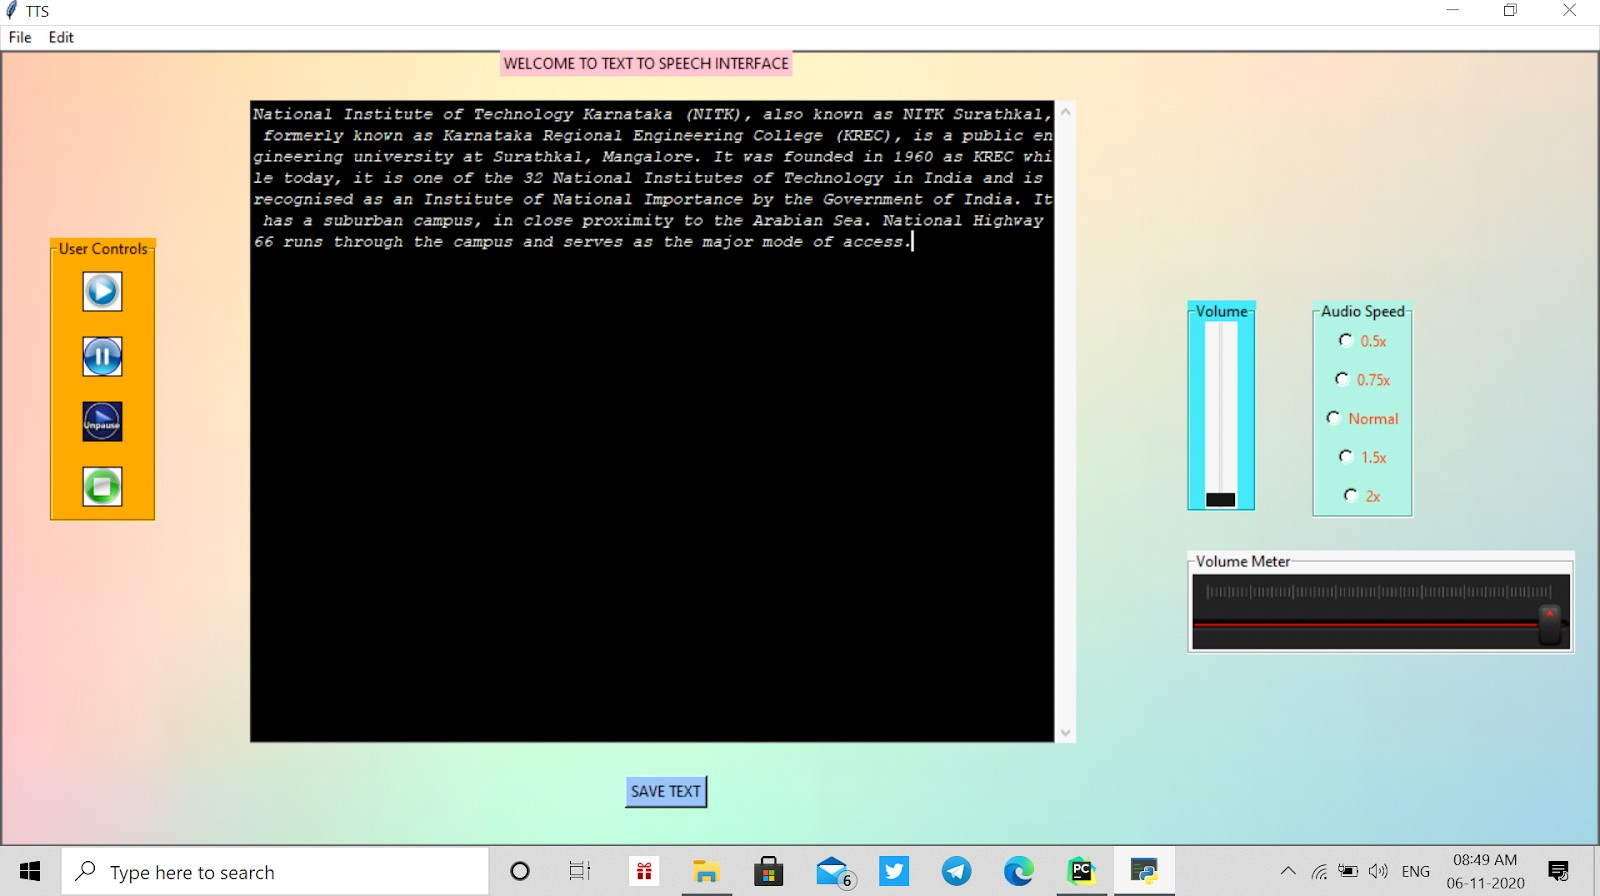
\includegraphics[width=3.01265in,height=1.68000in]{image11.jpeg}

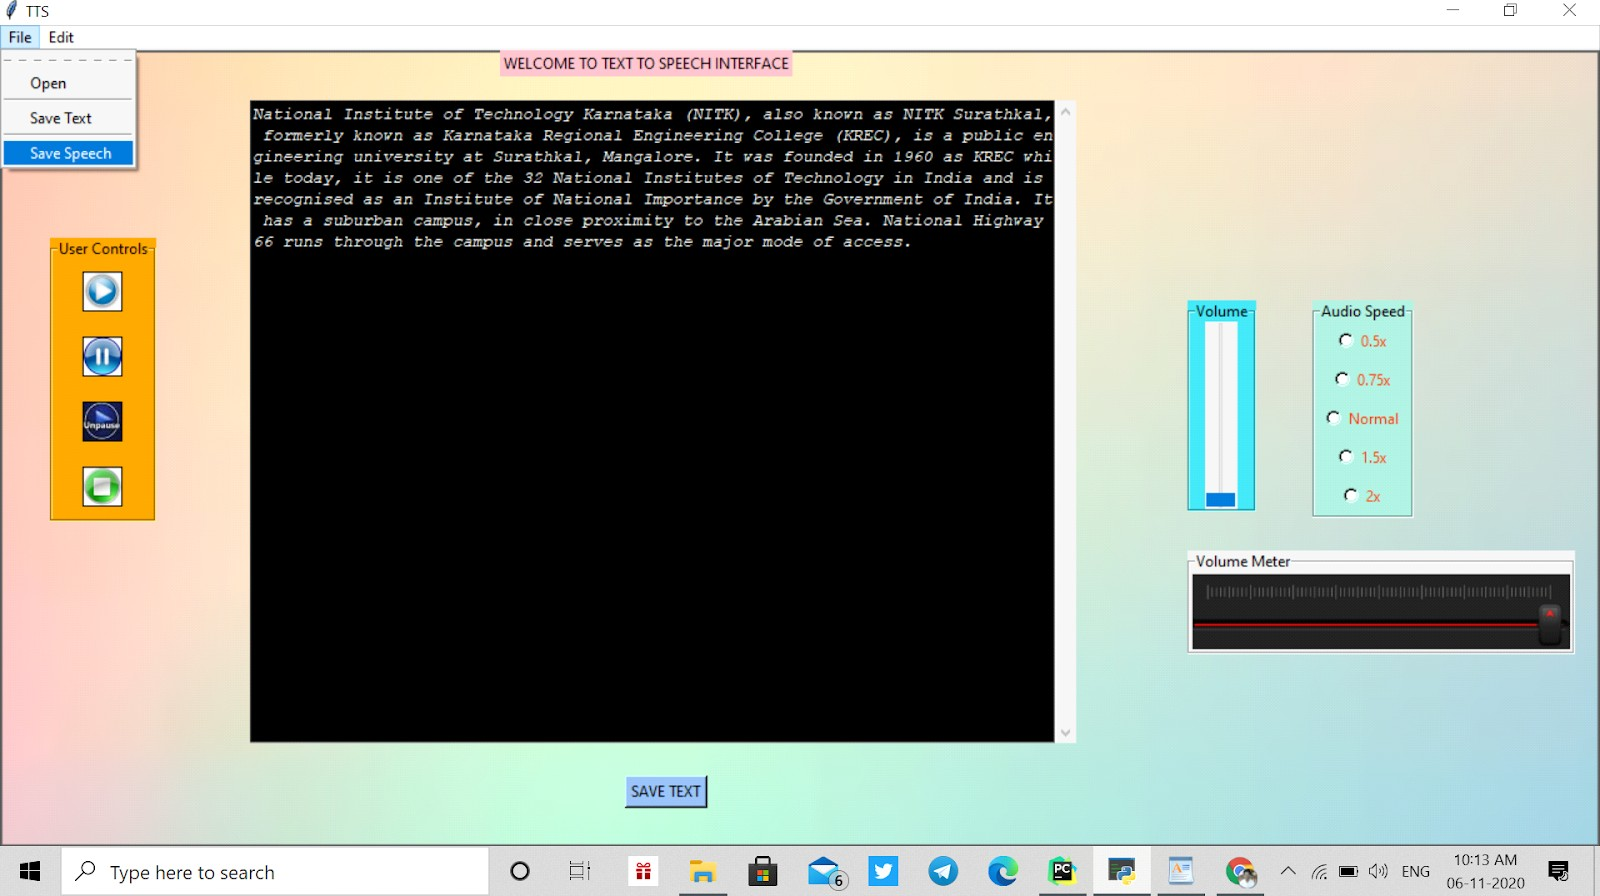
\includegraphics[width=3.08263in,height=1.86667in]{image12.jpeg}

\begin{quote}
If we want to save the speech just goto File menu and click the Save
Speech command.

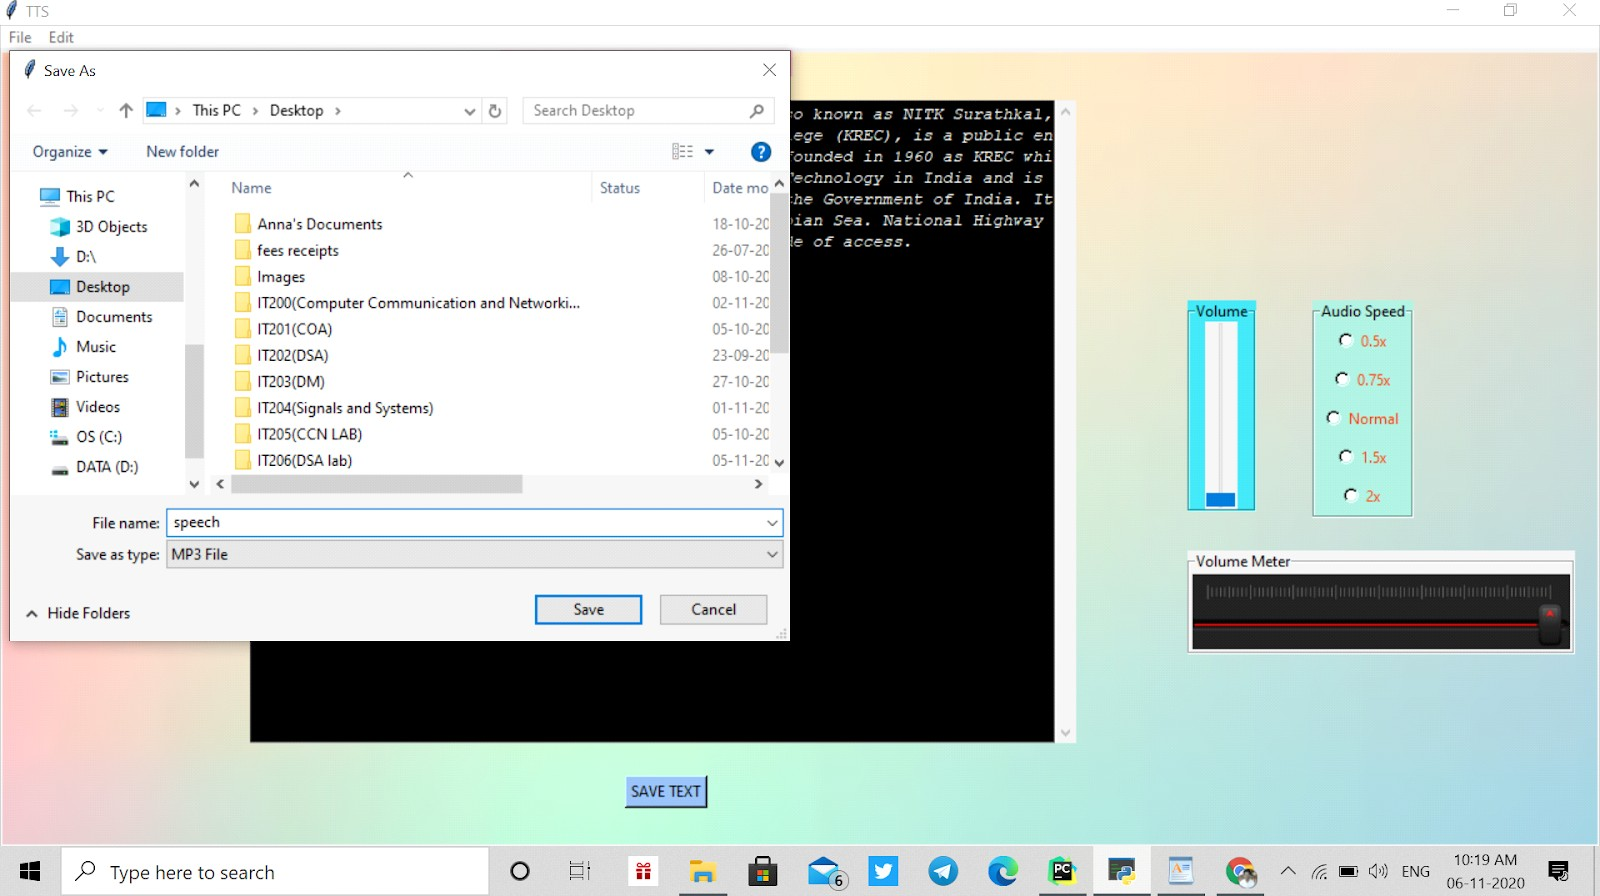
\includegraphics[width=3.29506in,height=1.96000in]{image13.jpeg}

AGer clicking on the Save speech button the new window will open named
as Save As there you can select any directory where you want to save the
audio file and give the file name and click on the save button.
\end{quote}

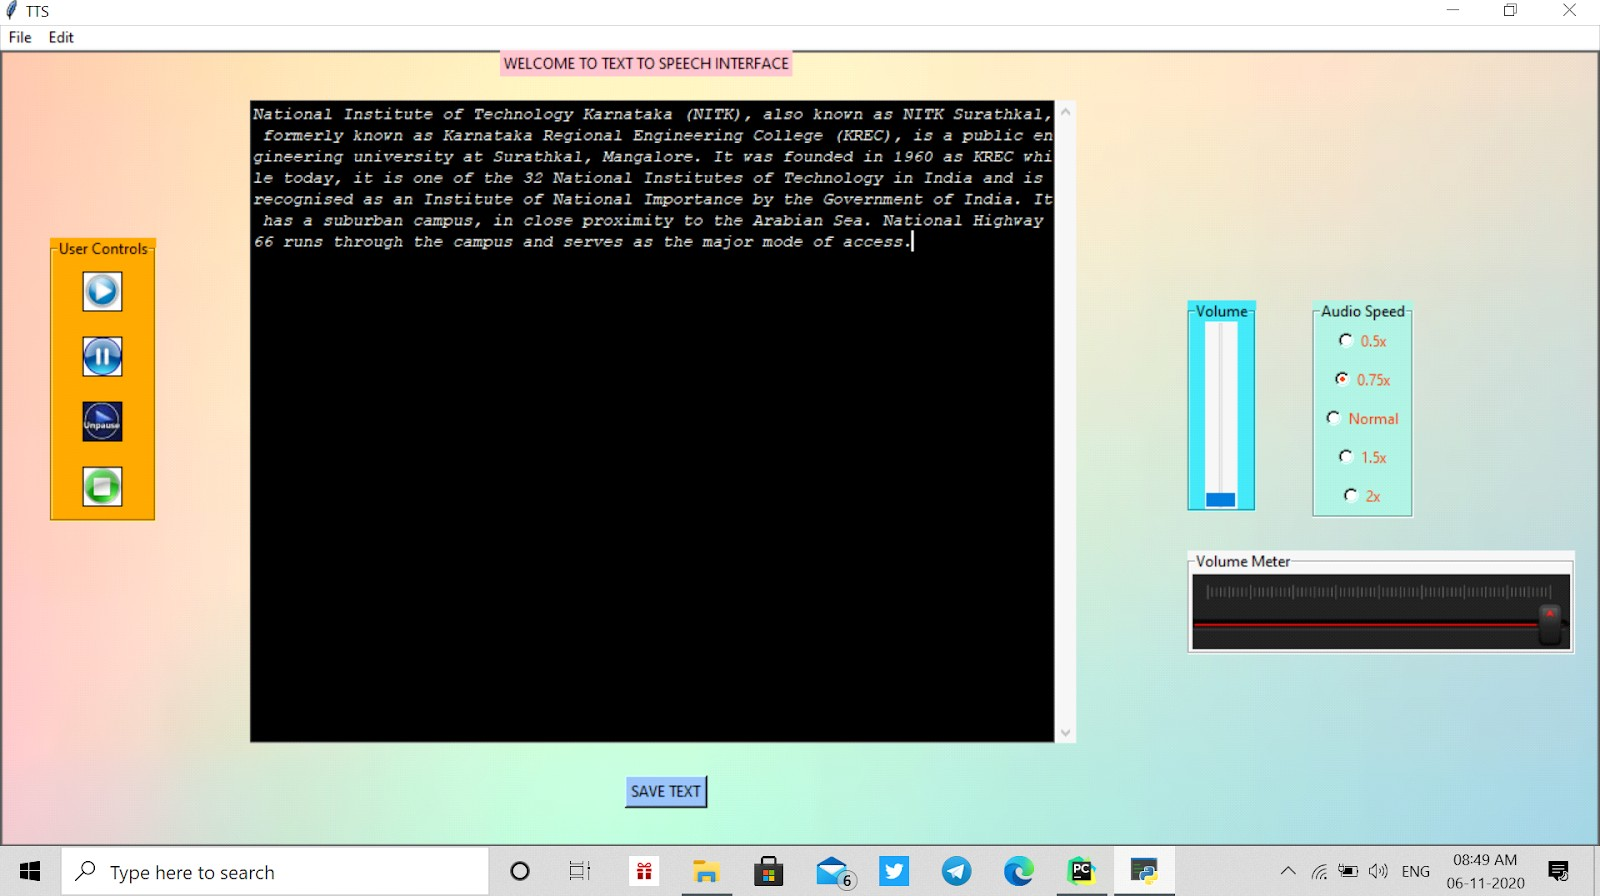
\includegraphics[width=3.06367in,height=1.96000in]{image14.jpeg}

\begin{quote}
To change the Speech speed click on the options which are present in the
Audio Speed LabelFrame.
\end{quote}

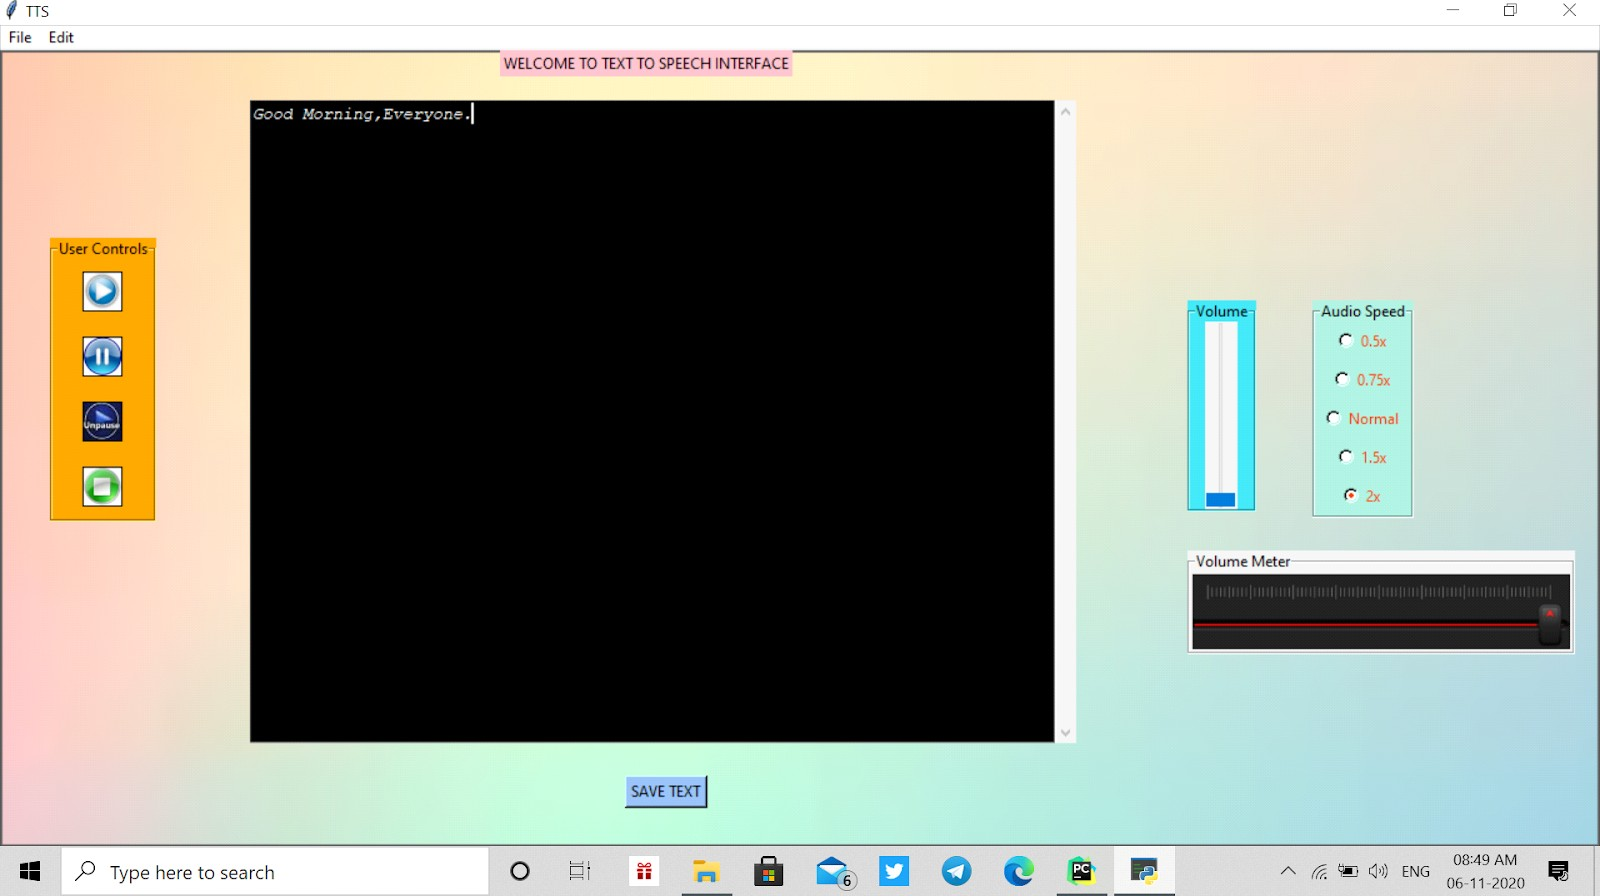
\includegraphics[width=3.03125in,height=1.86667in]{image15.jpeg}

\begin{quote}
The other option for filling a text Field is by writing anything into the
given Text Field.

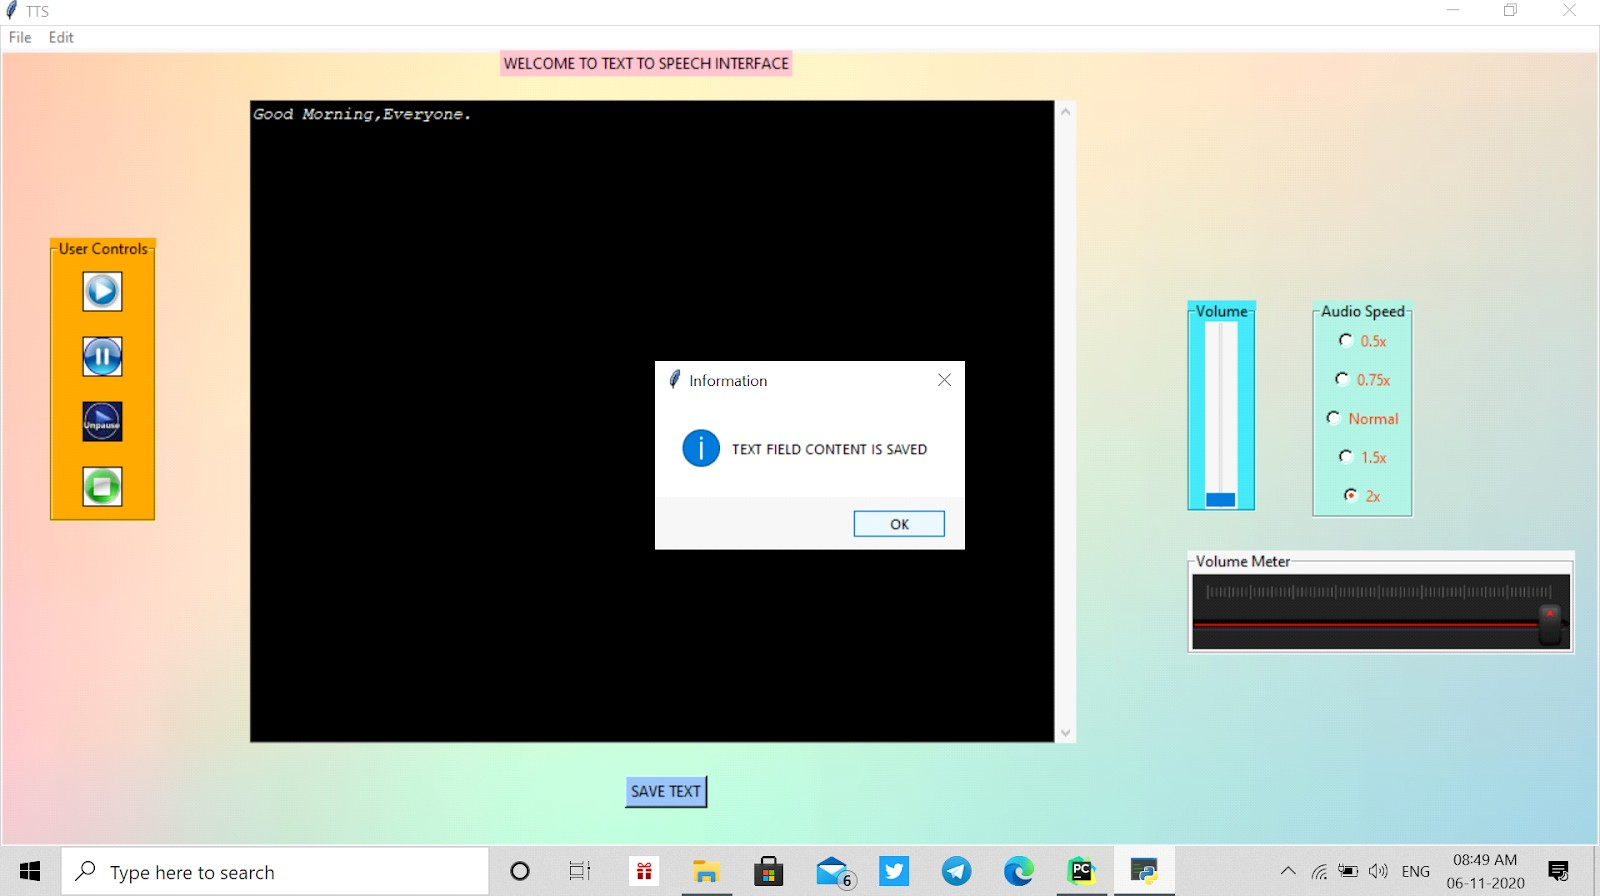
\includegraphics[width=3.10386in,height=1.77333in]{image16.jpeg}

Once you stop writing in the text field click on the save text button
which is just below the text field to save the content present in the
text field.
\end{quote}

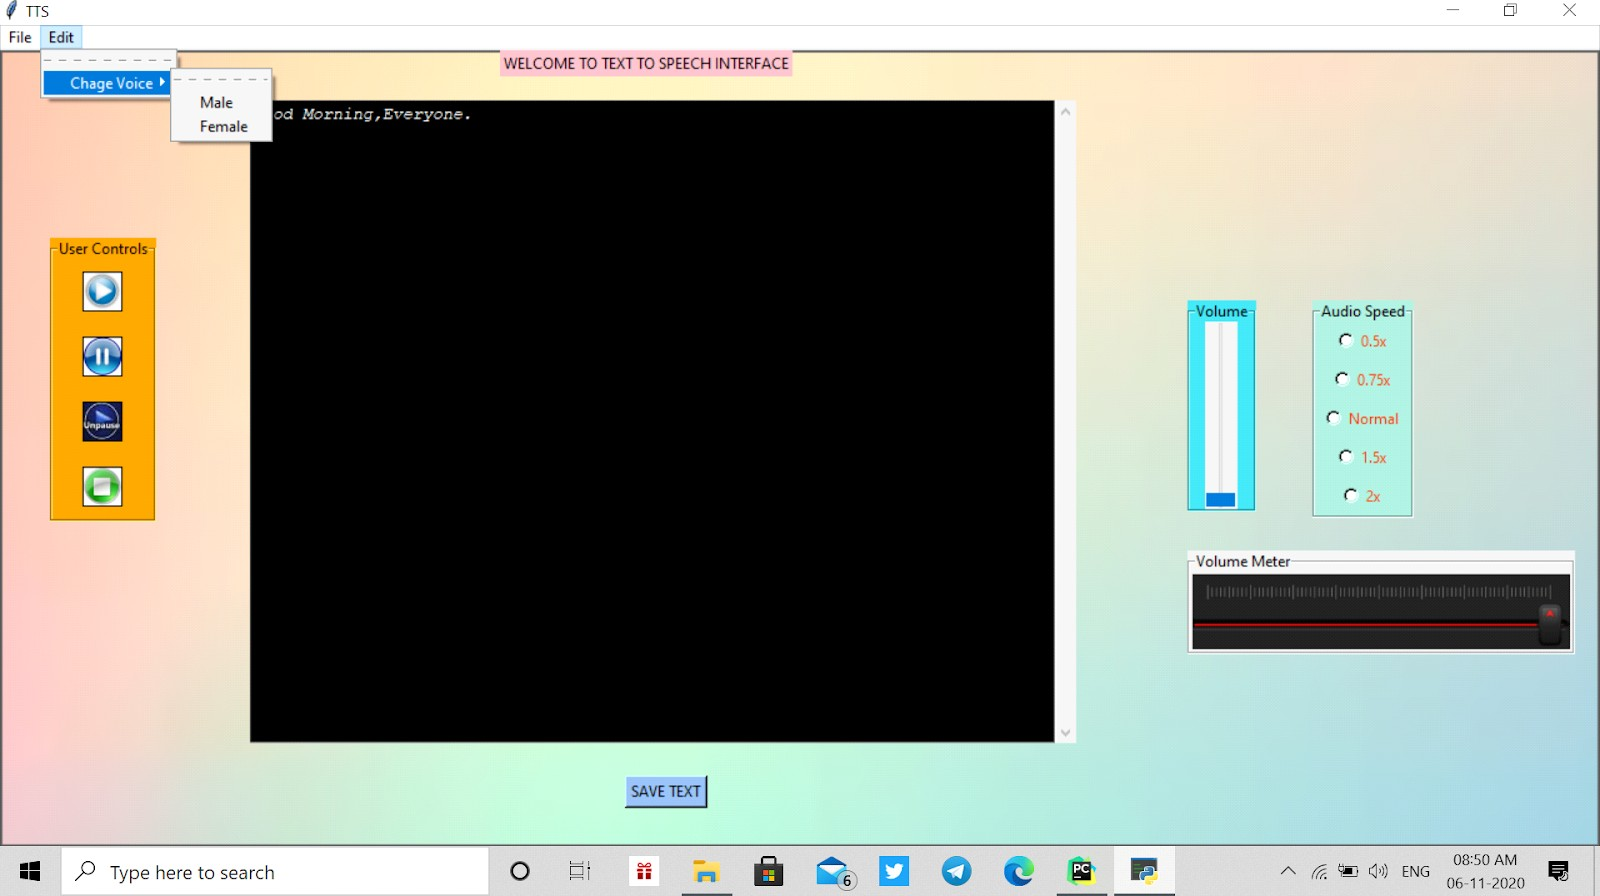
\includegraphics[width=2.99428in,height=1.68000in]{image17.jpeg}

\begin{quote}
Here in the Edit menu bar we can see the change voice command which is
used to change the voice to male and female.Click male to change the
voice from female to male and vice-versa.
\end{quote}

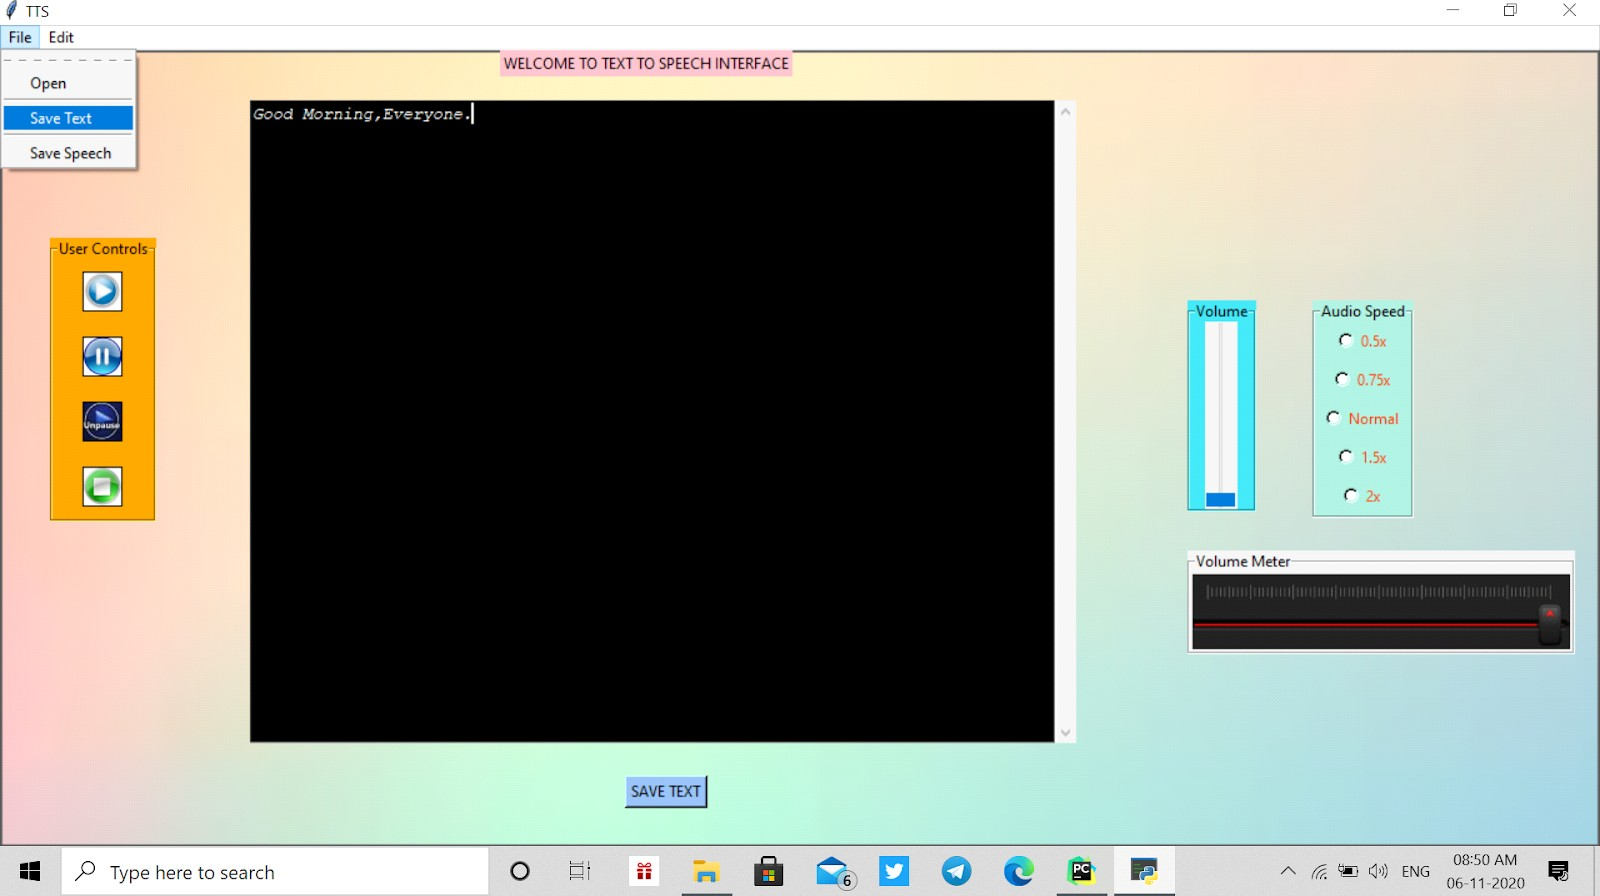
\includegraphics[width=2.99429in,height=1.68000in]{image18.jpeg}

\begin{quote}
To save the content from the text field goto File menu and click on the
save Text command.

AGer clicking on the Save Text button the new window will open named as
Save As there you can select any directory where you want to save the
Text file and give the file name and click on the save button.

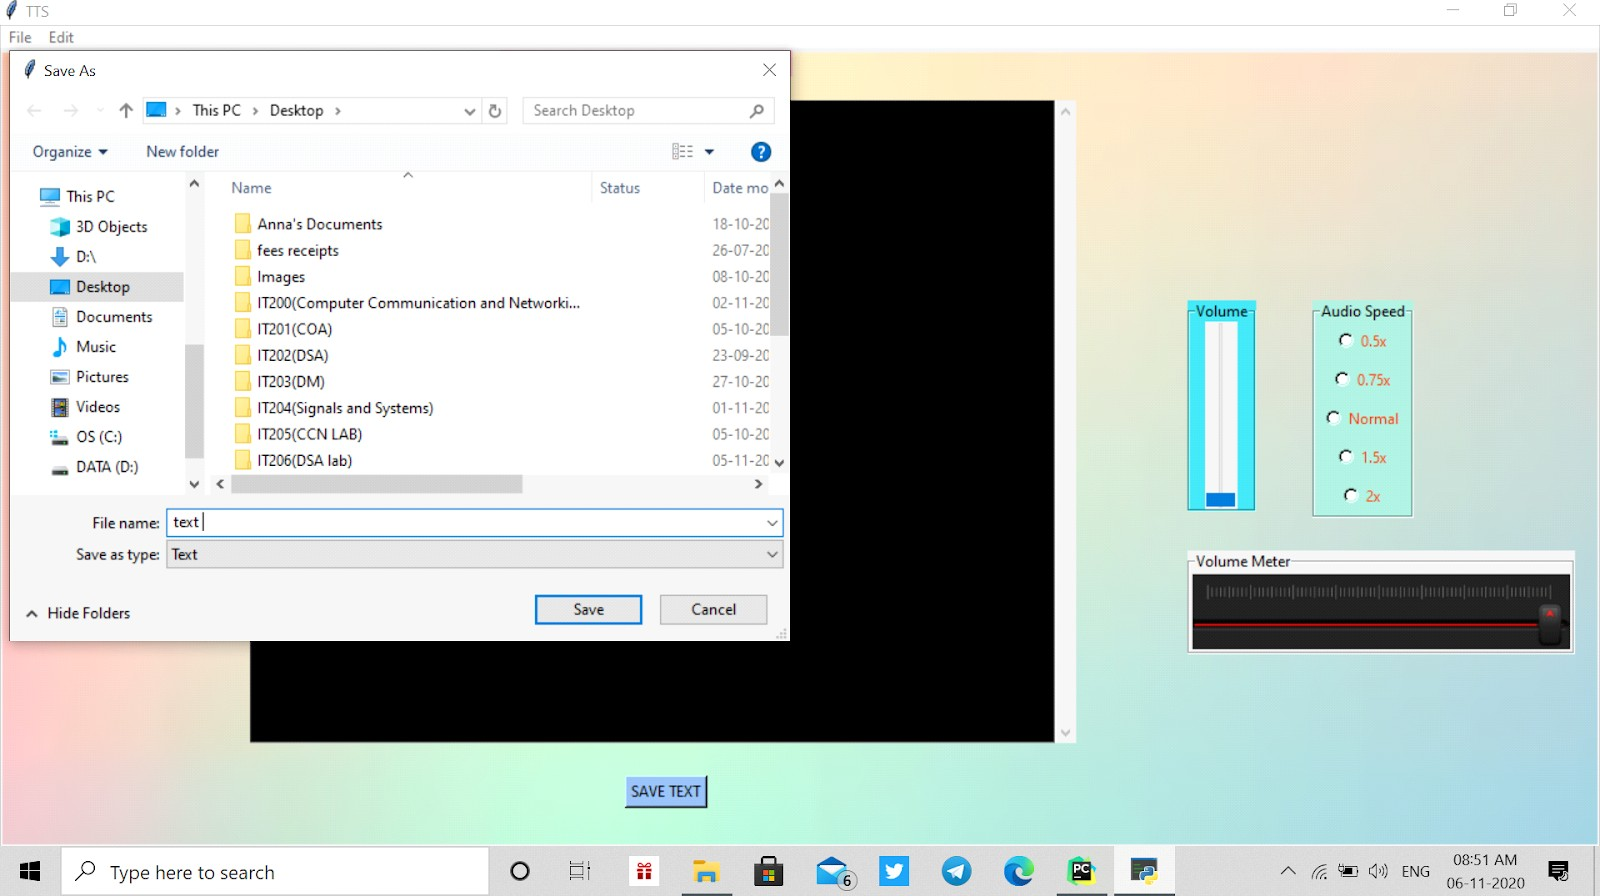
\includegraphics[width=3.02870in,height=2.08269in]{image19.jpeg}\textbf{STT}
\end{quote}

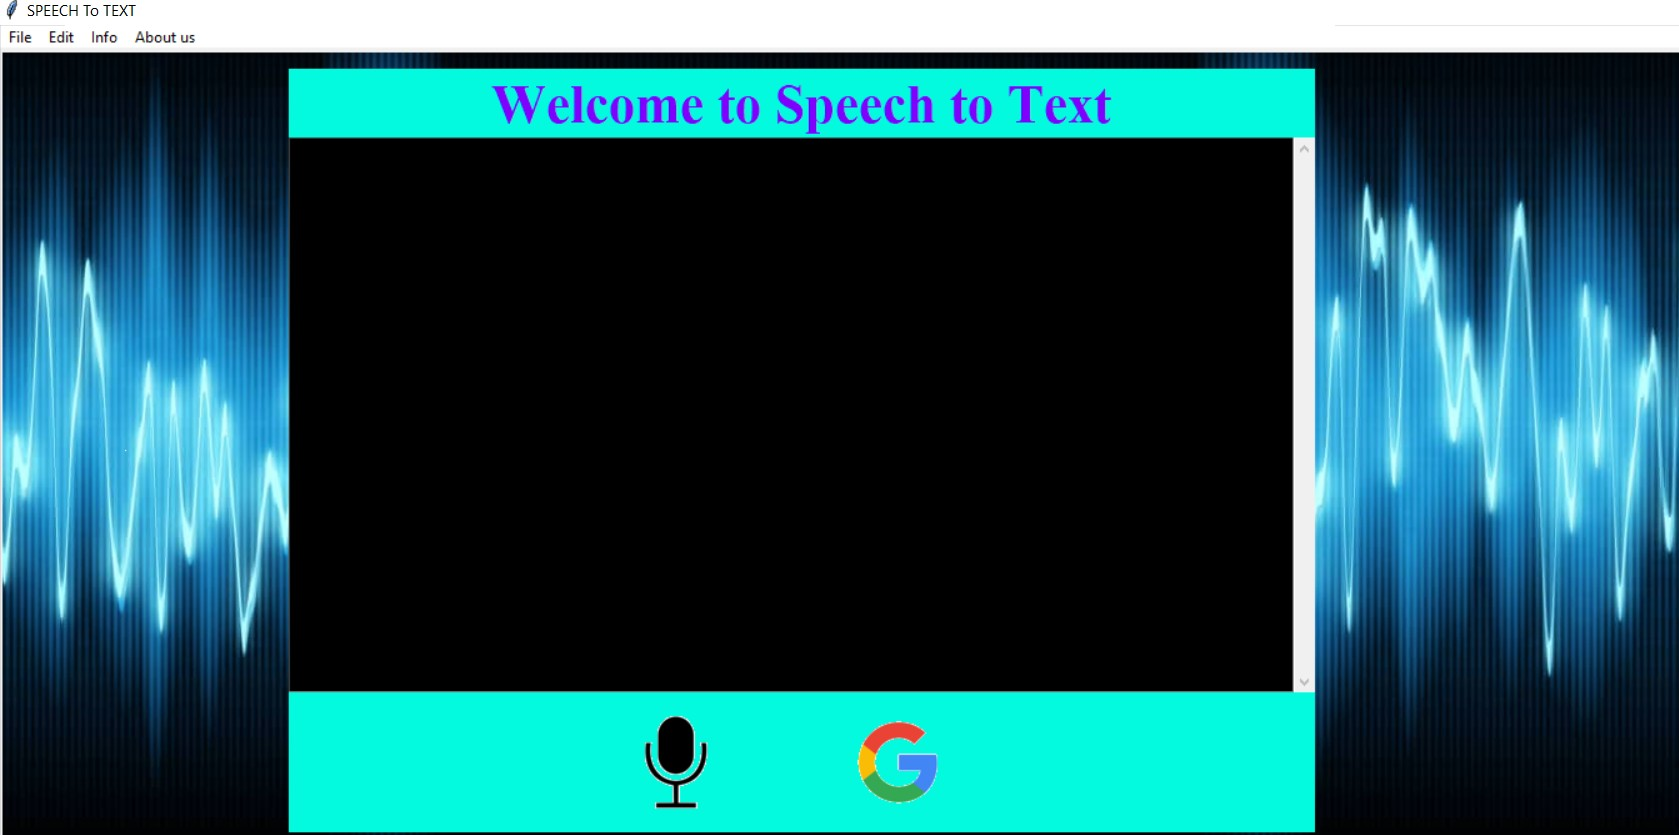
\includegraphics[width=3.50618in,height=1.73958in]{image20.jpeg}

\begin{quote}
This is a gui for speech to text.It contains a text field, canvas and
button widgets. It also has menu bar
\end{quote}

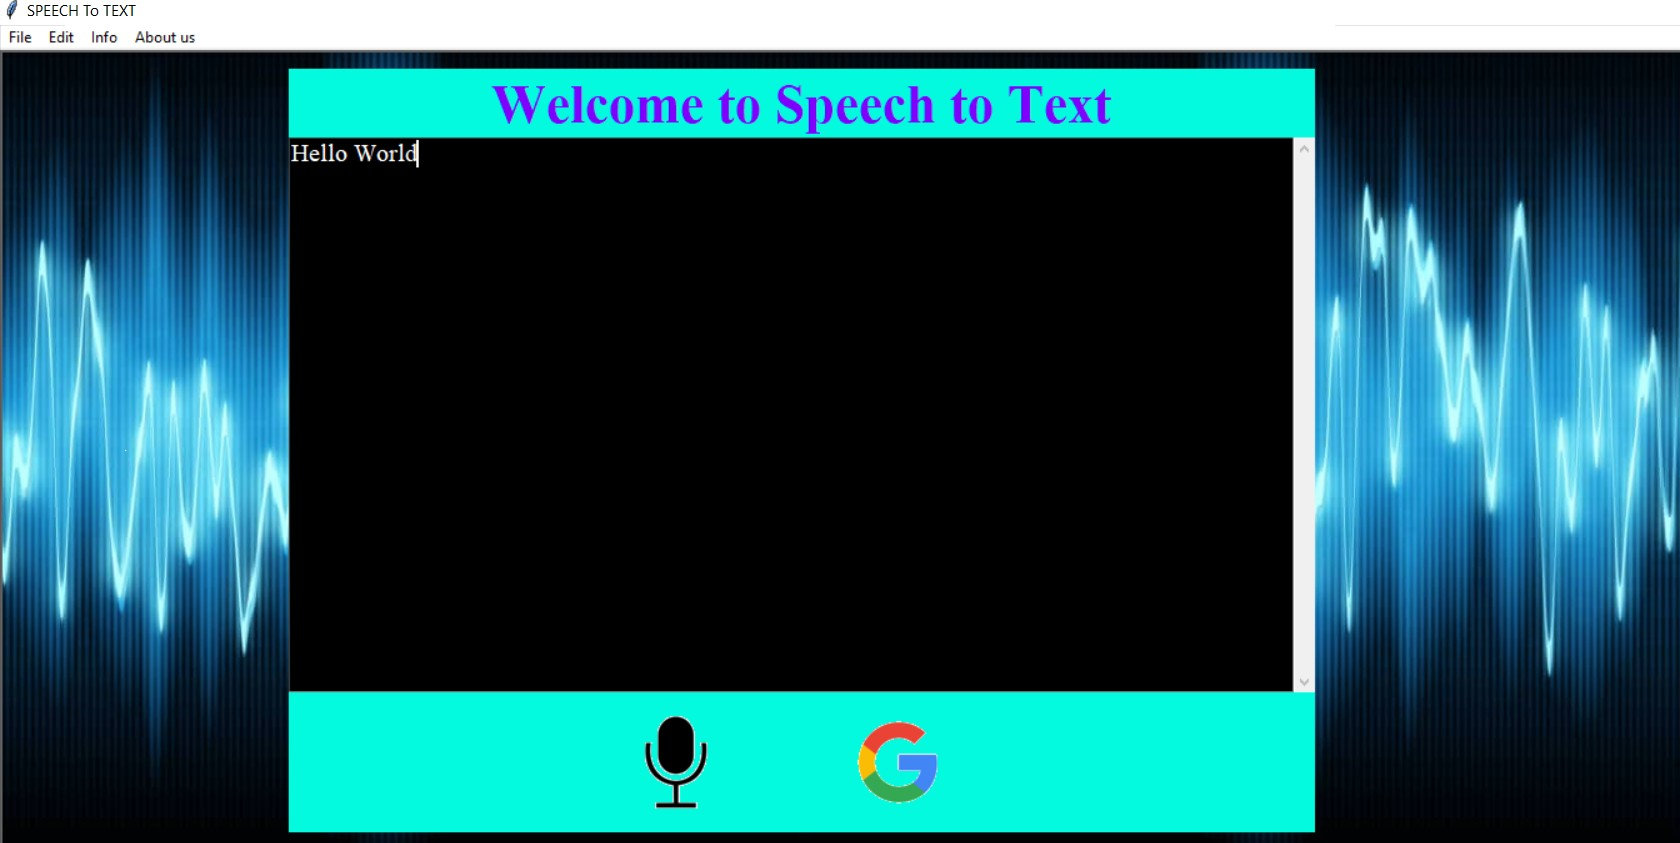
\includegraphics[width=3.49821in,height=1.75625in]{image21.jpeg}

\begin{quote}
AGer pressing the microphone button, the system will output an audio
signal saying speak now. AGer this user can give speech input. This
speech signal is converted to text and displayed in the Text Field.
\end{quote}

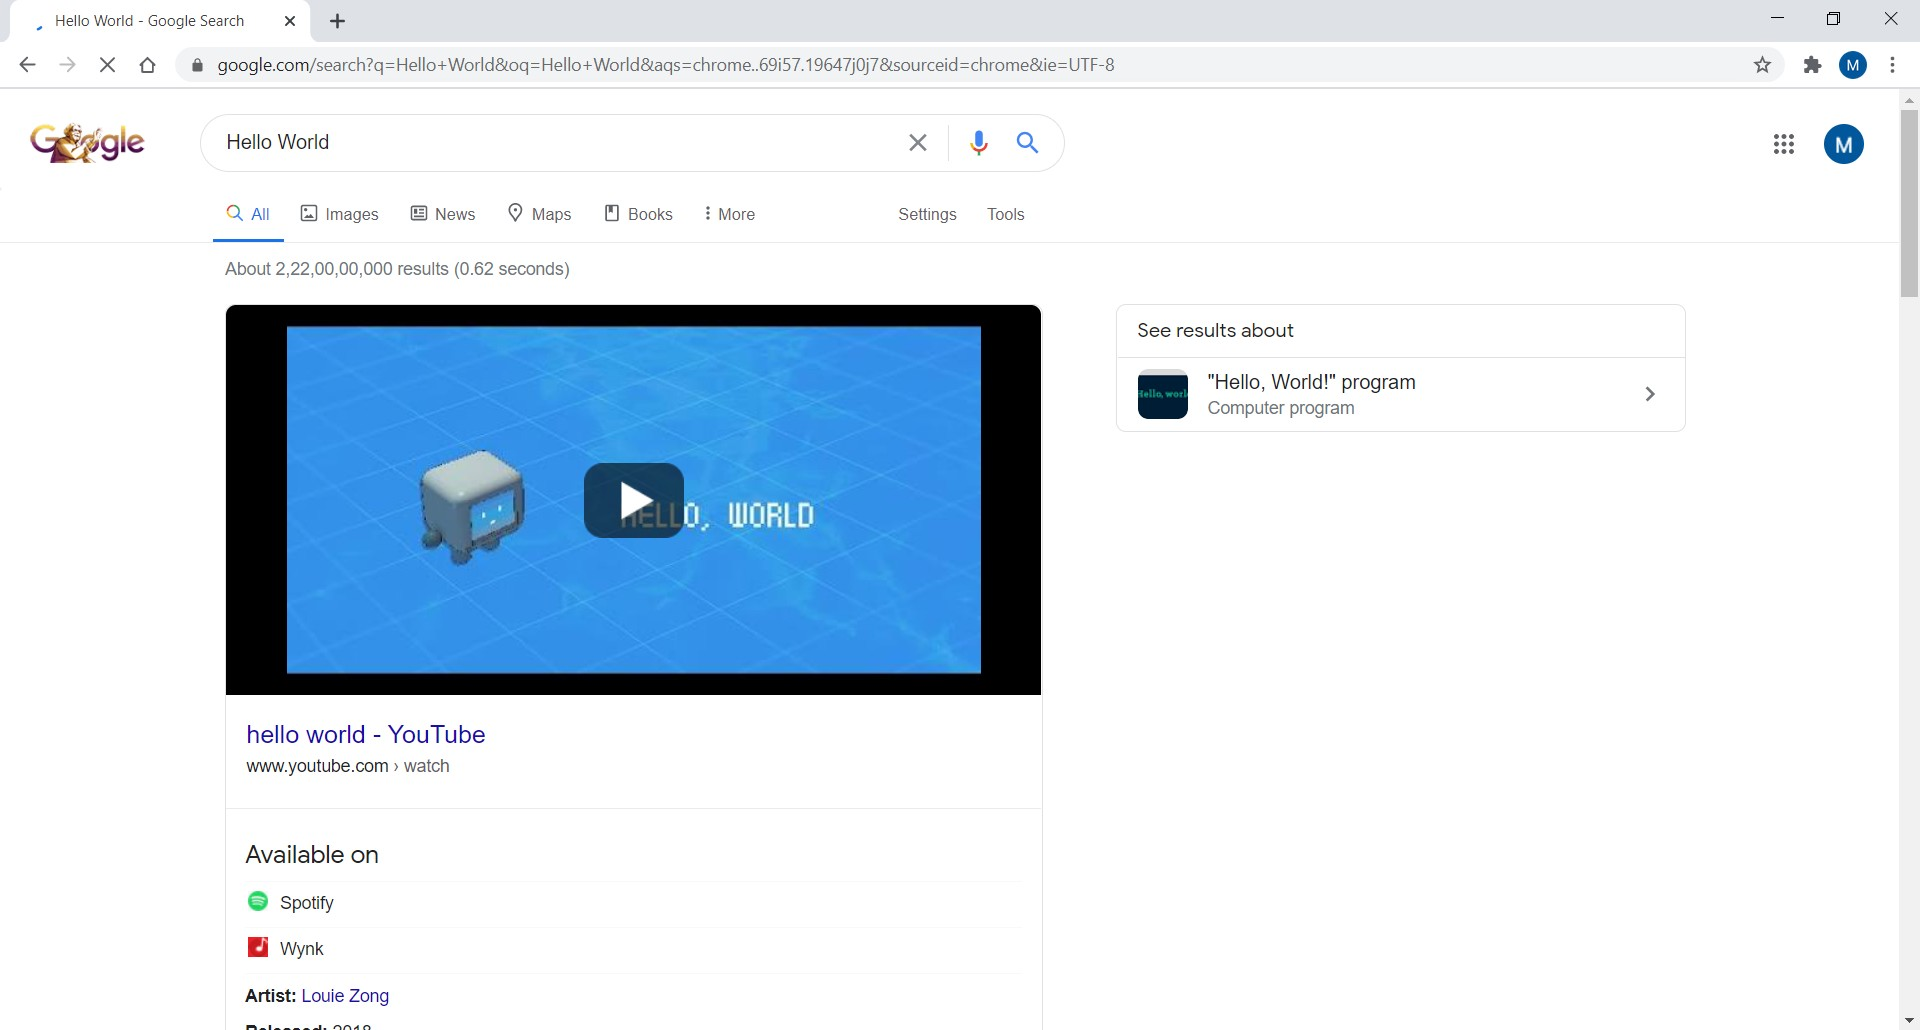
\includegraphics[width=3.41615in,height=1.82396in]{image22.jpeg}

\begin{quote}
This opens a new tab in browser which searches web for contents in our
text field

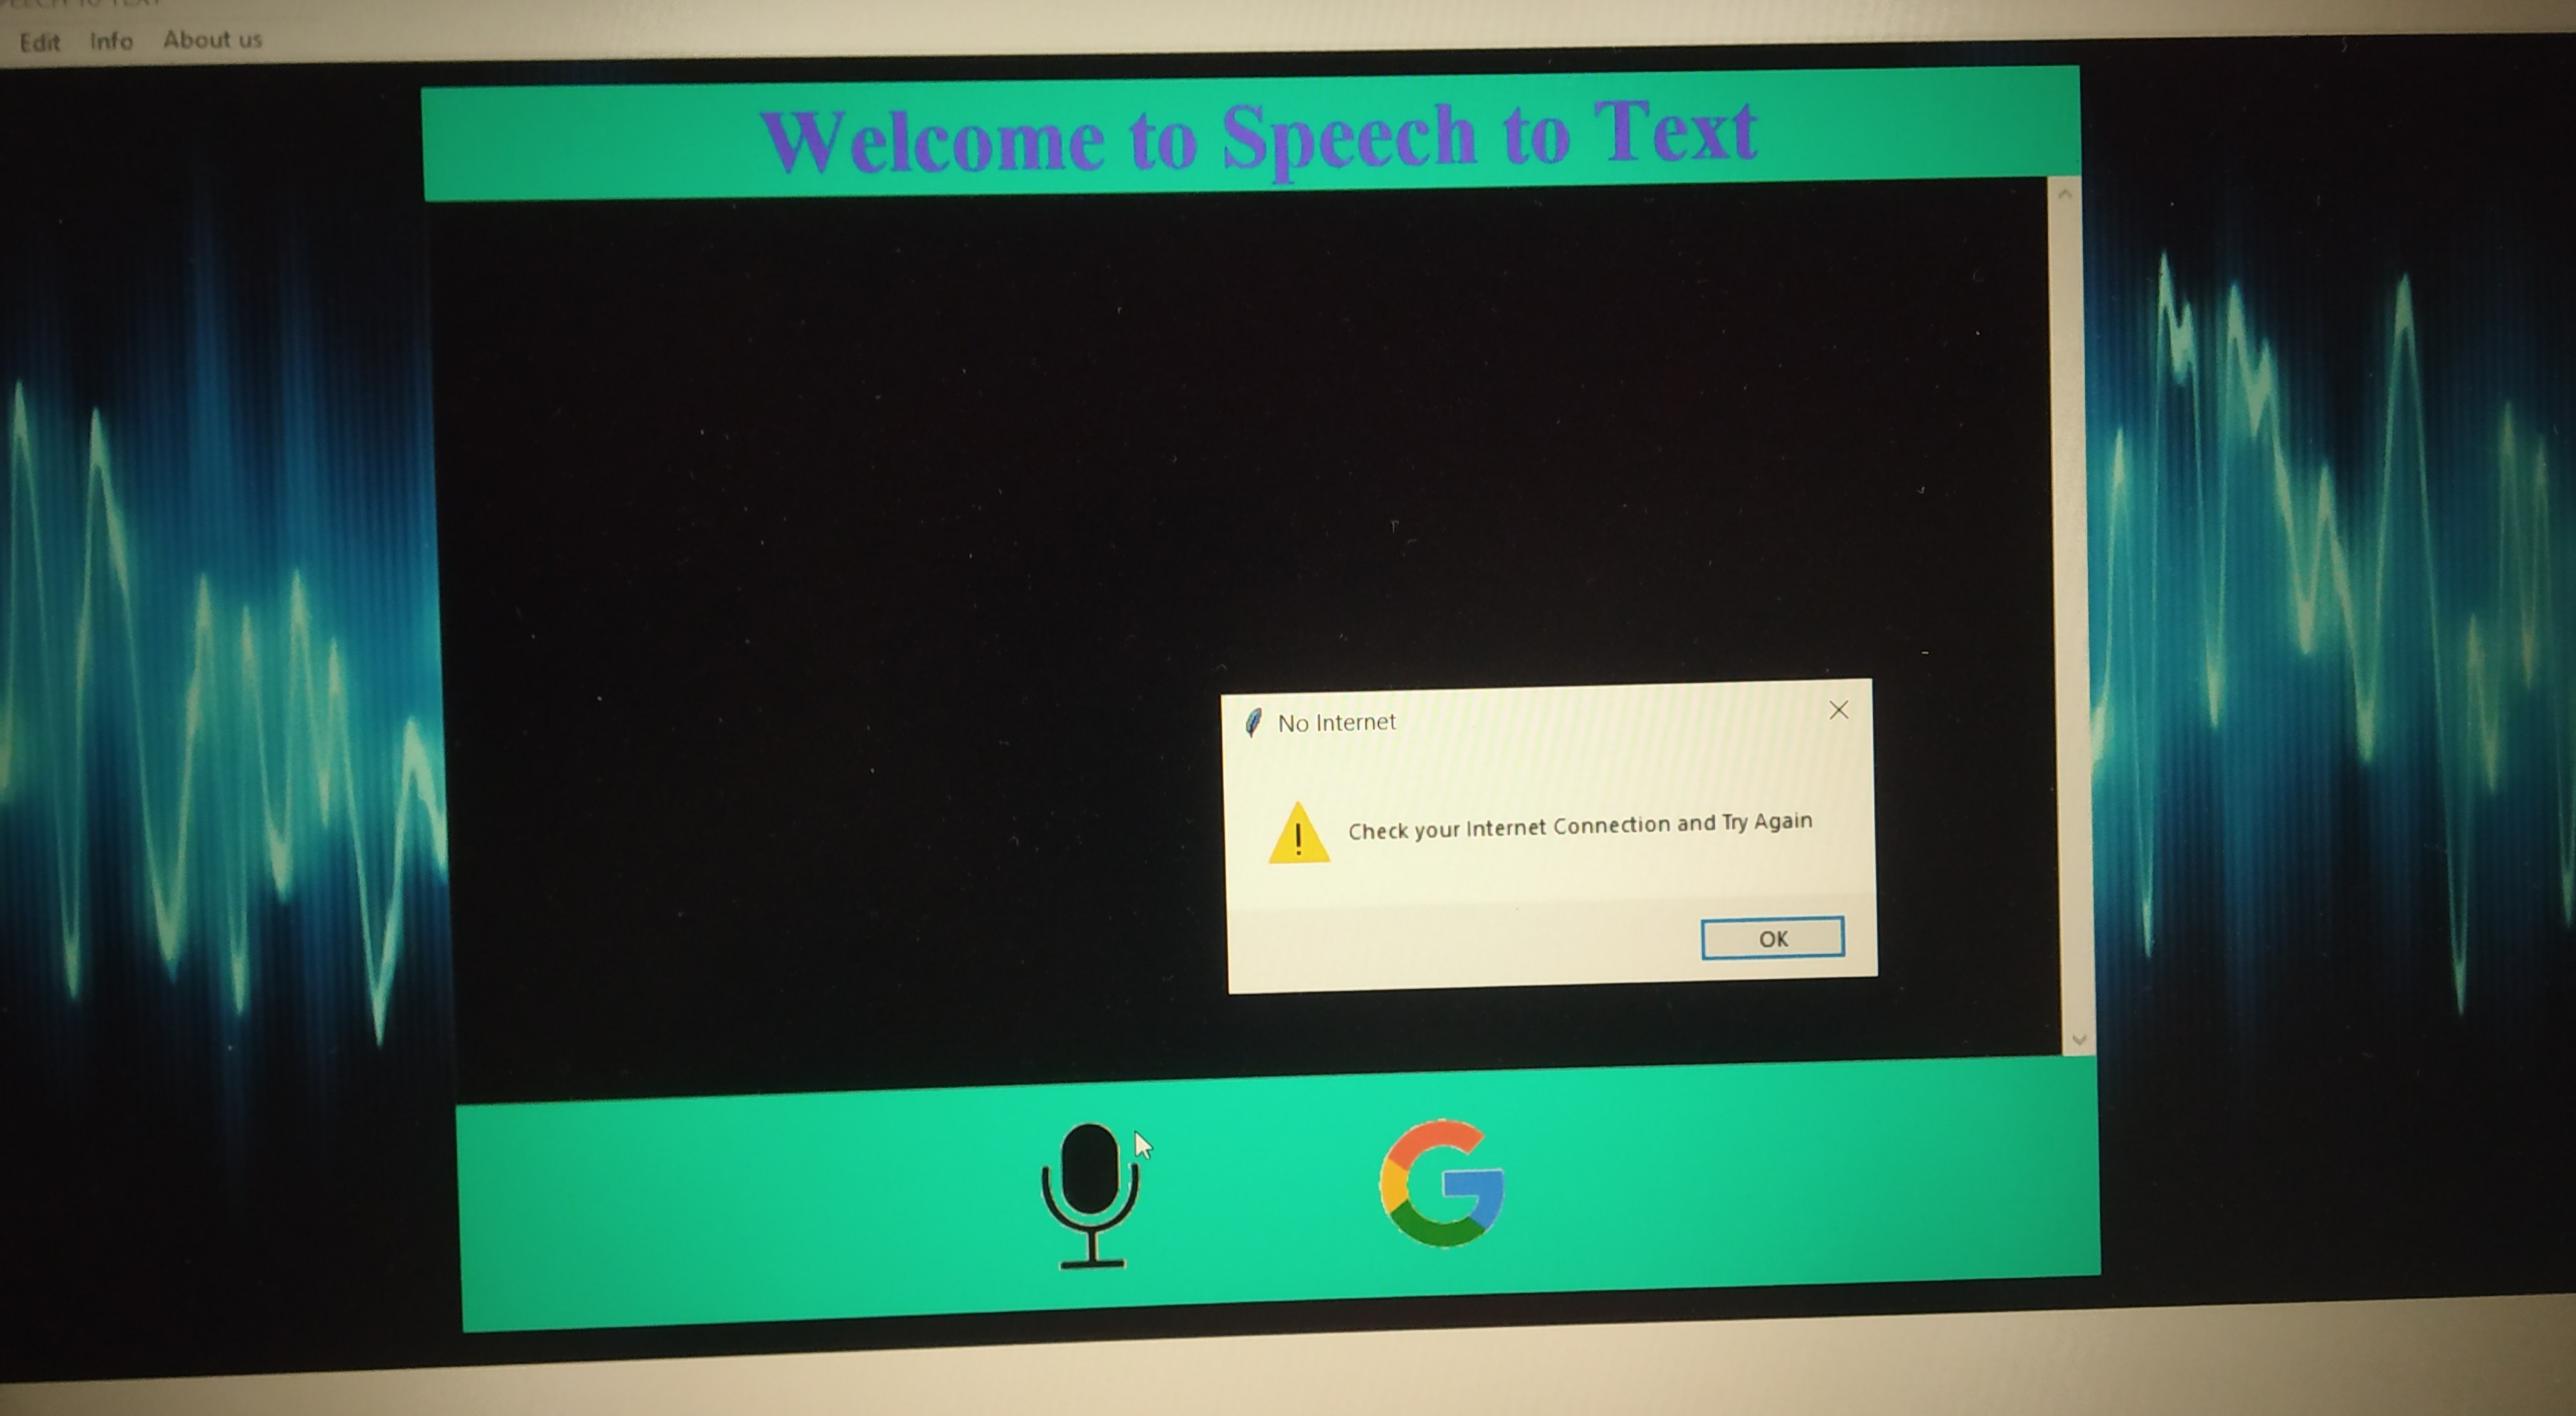
\includegraphics[width=3.38207in,height=1.86562in]{image23.jpeg}

While speaking if user is not connected to internet a window pops up
addressing the issue
\end{quote}

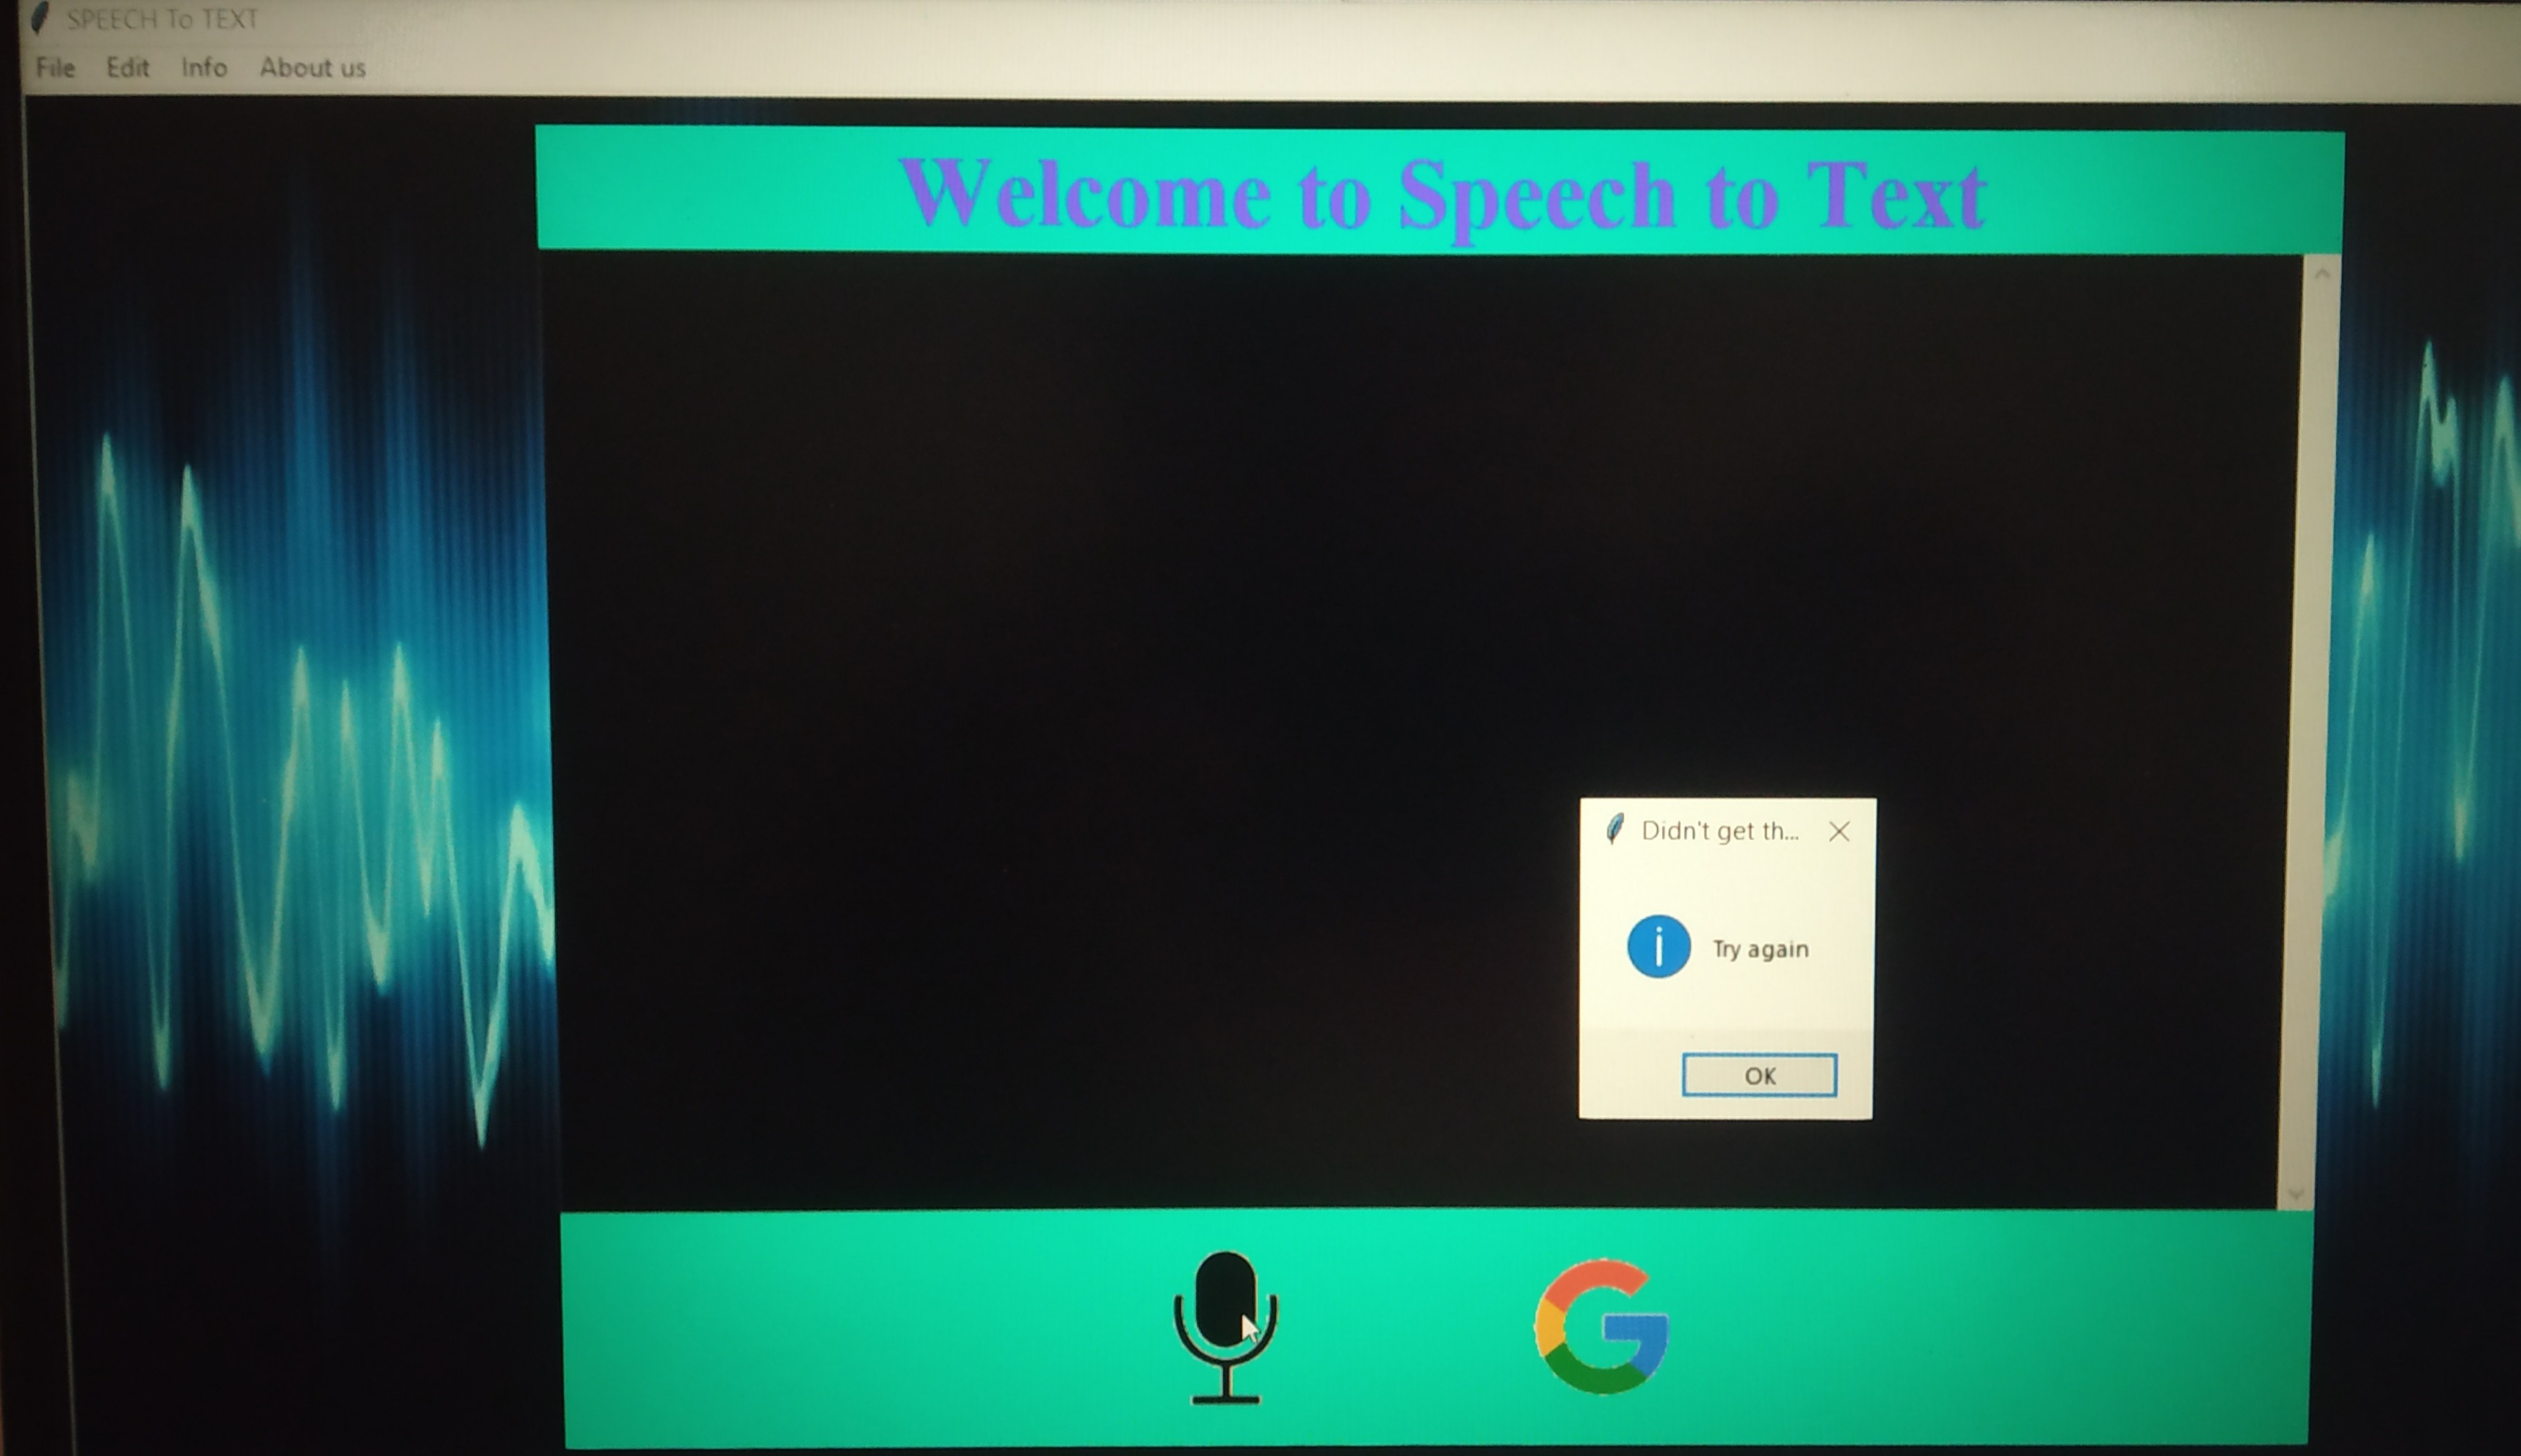
\includegraphics[width=3.41973in,height=1.97719in]{image24.jpeg}

\begin{quote}
If recognizer don't understand user's input this window pops up
addressing the issue
\end{quote}

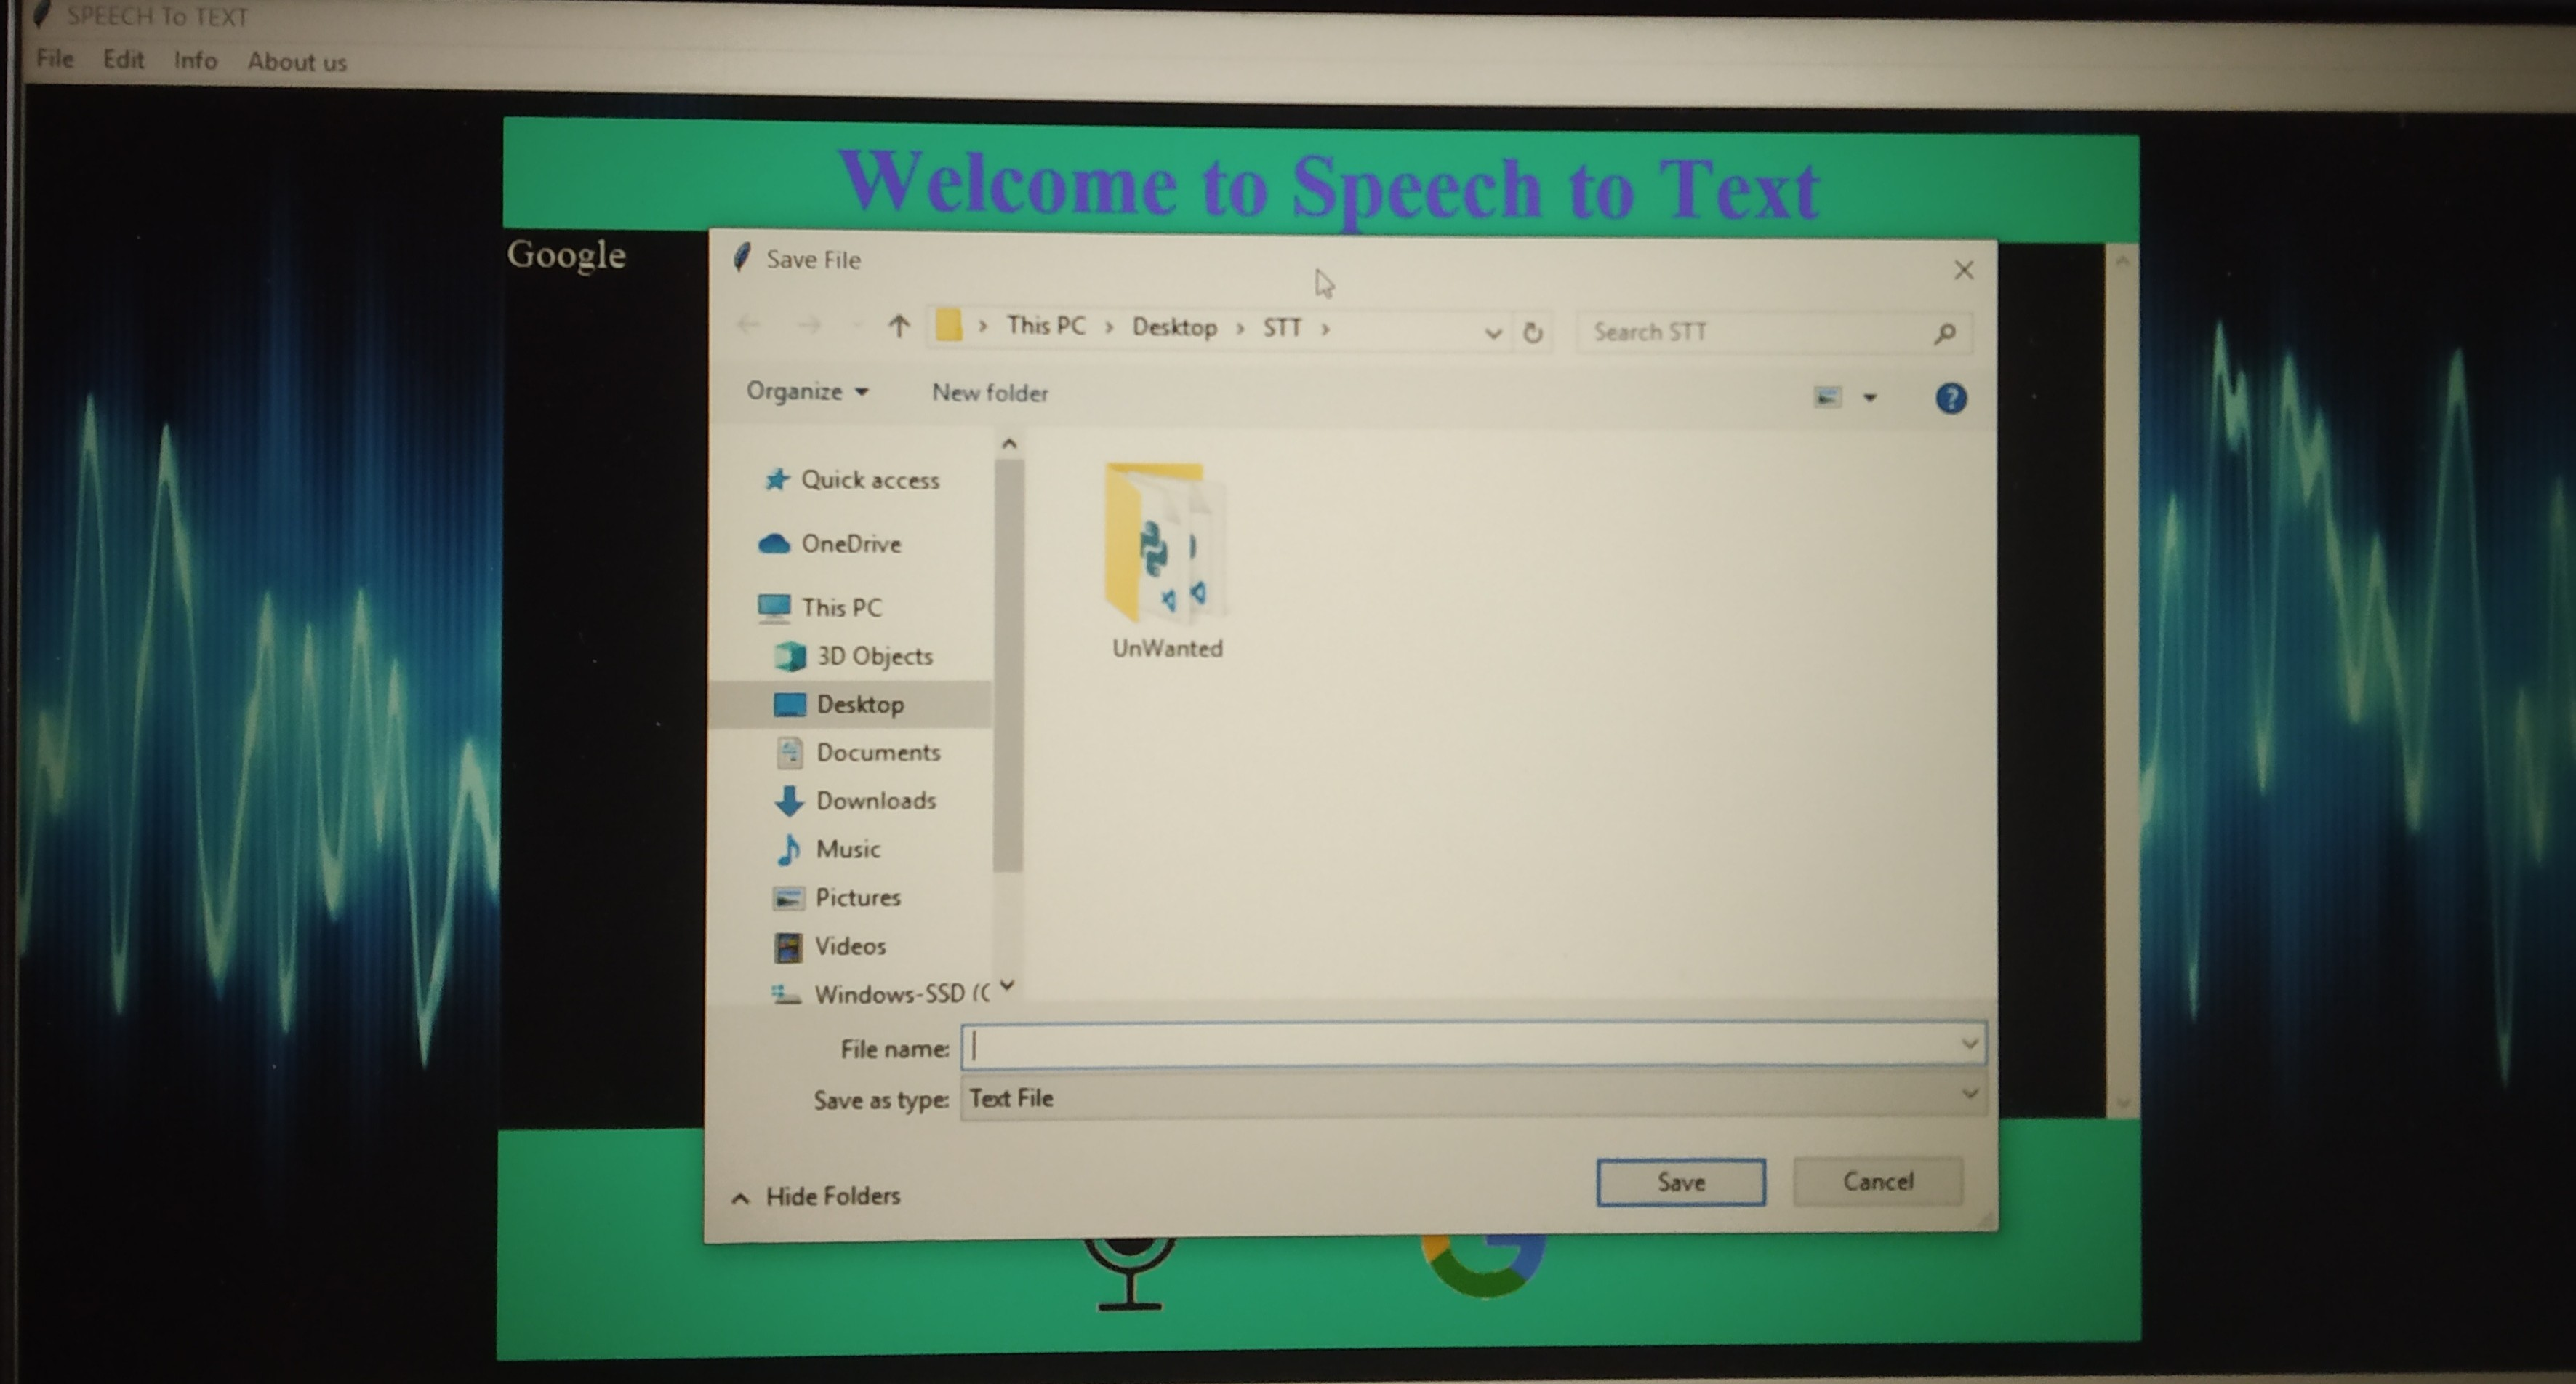
\includegraphics[width=3.33911in,height=1.58583in]{image25.jpeg}

\begin{quote}
Save and Save As options save files on the computer while Exit options
closes our application. We can save our output in the text field using
the save in file menu. The supported formats are .txt, .py ,.html

The clear button clears contents in the text field.

The info button in info menu shows guide to operate the application.The
about us button gives information about developers

\textbf{FEEDBACK:}

We shared our application with people and via google survey forms ,we
obtained many responses including positive and negative reviews.Most of
the outline of it were as follows:
\end{quote}

\paragraph{\texorpdfstring{\\
POSITIVE:}{ POSITIVE:}}\label{positive}

\begin{itemize}
\item
  No internet use in TTS so it can be useful in rural or remote areas.
\item
  In rural areas this concept is very new and by proper implementation
  ,it can make the edge in doing the easiness of their work.
\item
  Record of audio files can be maintained in TTS
\item
  The STT option of google is available.
\end{itemize}

\begin{quote}
\textbf{NEGATIVE:}
\end{quote}

\begin{itemize}
\item
  Slow working of STT application.
\item
  Internet usage in STT application.
\item
  No option available to change the speed of the audio file in TTS.
\end{itemize}

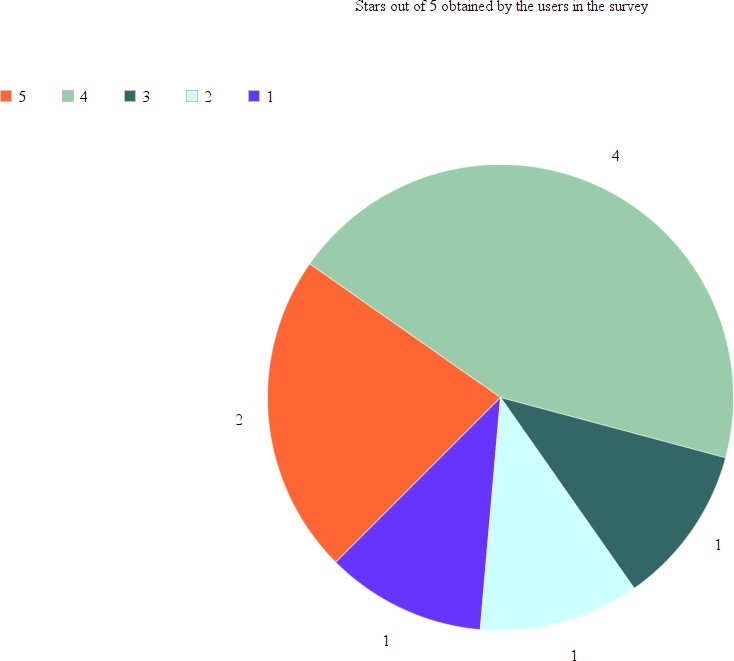
\includegraphics[width=2.06238in,height=1.99677in]{image26.jpeg}

\section{Conclusion:}\label{conclusion}

\begin{quote}
Text-to-Speech synthesizers have steadily developed from the last few
decades to gain the current shape. It's never been so easy to use a
text-to-speech program, as just one click and your computer will speak
any text aloud in a clear, natural sounding voice. We have identified the
various operations and processes involved in text to speech synthesis.
We have also developed a very simple and attractive graphical user
interface which allows the user to type in his/her text provided in the
text field in the application. Our system interfaces with a text to
speech engine developed for American English.We have also implemented it
successfully in the marked needy areas.Also in future we will be trying
it to add more and more regional and international languages so that
linguistic barrier will be demolished.Also for speech to text converter
we will try to make it completely offline.
\end{quote}

\section{CONTRIBUTION:}\label{contribution}

\subsection{Work done:}\label{work-done}

\begin{itemize}
\item ~
  \subsubsection{STT}\label{stt}
\end{itemize}

\begin{enumerate}
\def\labelenumi{\arabic{enumi}.}
\item
  Anshul: Draw outline of gui and build start window.
\item
  Mohit: Implement the conversion from speech to text(core)
\item
  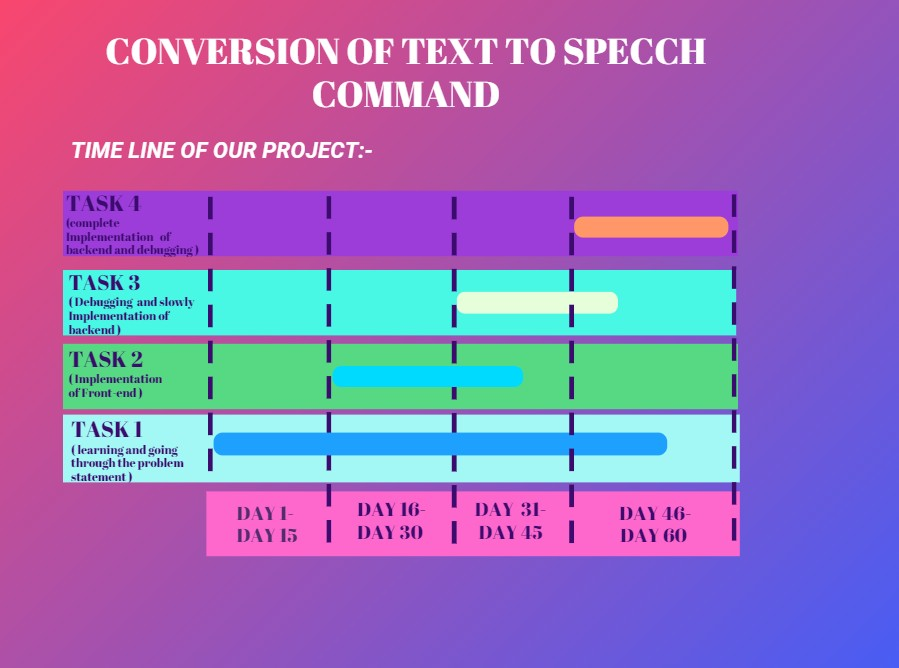
\includegraphics[width=3.27849in,height=2.59157in]{image27.jpeg}Rakshit:
  Build menu and 2 buttons on welcome screen and exception handling in
  conversion from speech to text
\item
  Kiran: Implement command for all options in the menu namely save,
  saveas, clear, exit, info and about us.
\end{enumerate}

\begin{itemize}
\item ~
  \subsubsection{TTS}\label{tts}
\end{itemize}

\begin{quote}
First we all studied the referenced papers and we spent some time
understanding the problem statement and its related things.AGer that we
started making our GUI. The GUI contains FrontEnd and BackEnd.
\end{quote}

\begin{enumerate}
\def\labelenumi{\arabic{enumi}.}
\item
  \textbf{Mohit}

  \begin{itemize}
  \item
    Creating window and adding menu
  \end{itemize}
\end{enumerate}

\begin{quote}
bar(Front End) -
\end{quote}

\begin{itemize}
\item
  He worked with Volume Slider i.e how to change the volume and
  corresponding to volume how volume Meter will change and also how to
  change the audio speed. (Back End)
\end{itemize}

\begin{enumerate}
\def\labelenumi{\arabic{enumi}.}
\setcounter{enumi}{3}
\item
  \textbf{\\
  Rakshit}

  \begin{itemize}
  \item
    Creating a Scrolled Text field and saving the text button. (Front
    End)
  \item
    He worked with the User Control LabelFrame which consists of play
    pause unpause and stop button. (Back End)
  \item
    He also did all the testing.
  \end{itemize}
\end{enumerate}

\begin{enumerate}
\def\labelenumi{\arabic{enumi}.}
\setcounter{enumi}{1}
\item
  \textbf{Anshul}

  \begin{itemize}
  \item
    Creating User Control LabelFrame and adding play , pause, unpause
    and stop button (Front End)
  \item
    File menu bar contains sub menu bars open,save speech and save text
    and Edit menu bar contain change voice command. (Back End)
  \end{itemize}
\item
  \textbf{Kiran}

  \begin{itemize}
  \item
    Creating Volume slider,Volume Meter and Audio speed controls. (Front
    End)
  \item
    He worked with Text Field like taking the input text and adding it
    into the Text box and also saving the text content as a .txt file.
    (Back End)
  \end{itemize}
\end{enumerate}

\end{document}